%%==================================================
%% chapter01.tex for BIT Master Thesis
%% modified by yang yating
%% version: 0.1
%% last update: Dec 25th, 2016
%%==================================================
% \chapter{基于分离-融合范式的多词元链接事件要素抽取模型}
\chapter{基于分离-融合范式的跨事件信息构建与利用}
\label{chap:chapter5}

以ACE2005数据集为代表的句子级别数据集被主流的事件抽取研究广泛采用,但随着真实世界文本内容的复杂性不断增加,事件要素信息越来越多地跨越出现在一个文档中的多个句子中。因此,研究同时适用于句子级别和文档级别事件要素抽取的通用模型成为新的研究热点和挑战。与上一章节不同,该研究遵循章节\ref{section2_2}所述的关于事件要素抽取的第二种定义,即不使用实体提及的标注信息,而在预测要素类型的同时识别出其文段范围。

现有通用文本级别事件要素抽取模型存在各自的局限性,而基于多词元链接的建模方法能够有效避免这些模型的内在局限,并展现出良好的性能潜力。因此,本章研究利用多词元链接方法进行通用文本级别的事件要素抽取。然而该方法中的单一事件建模方式缺乏对跨事件依赖关系的利用,多事件建模方式需要更长的要素类型序列编码和额外的链接操作,增加了预测推理的难度。为此,本章提出了一种基于分离-融合范式的跨事件信息构建与利用方法,并相应提出了一种新的多词元链接模型,避免了当前方法的各自局限,且实现了从不同级别文本中高效利用跨事件依赖信息。实验结果证明了本章提出的模型在所有句子级和文档级数据集上都优于目前性能最优的事件要素抽取模型。

\section{引言}
\label{introduction}

最近,基于抽取式~\cite{ma2022prompt, he2023revisiting, nguyen2023contextualized, li2023intra}和生成式~\cite{hsu2022degree,du2022dynamic,zhang2023overlap}的提示学习方法在同时适用于句子级别和文本级别的事件要素抽取任务上取得了显著的性能提升。然而,前者在抽取具有相同要素类型的多个事件要素时,受到提示模版中预先设定的重复要素槽位数量的限制,后者在抽取长距离事件要素的性能表现不佳。此外,这两类方法的性能表现均较为依赖于提示模版的设计质量。

因此,不同于基于提示学习的方法,最近的一些研究~\cite{wang2022query,lou2023universal,liu2023rexuie}将输入文本和所有涉及的要素类型串接成自然语言序列,然后联合编码,并进一步实施多词元\footnote{“词元”对应于英文表达中的“token”,这里特指经过预训练语言模型分词器分词后得到的语义单元。}链接操作,从而实现事件要素抽取或通用信息抽取的建模。其中,所有事件要素文段和要素类型的并行链接操作能够直接高效地抽取具有相同要素类型的多个事件要素,并提升长文本中分散的事件要素间的交互。此外,该类方法不需要精心设计的提示模版。根据每次同时抽取的事件数量,可以进一步将该类方法划分为两种建模方式:单事件抽取和多事件抽取。

第一种方式的研究~\cite{wang2022query,liu2023rexuie}将待抽取文本和只在目标事件中出现的要素类型串接后作为输入,然后实施两种链接操作去建模目标事件。如图\ref{example}所示,其中被红色标记的为事件触发词,被黄色标记的为事件要素类型,不同颜色的箭头表示不同种类的链接操作,事件要素“James McDade”在$Die$事件和$Attack$事件中扮演了不同的要素类型,其抽取建模过程是分离的。虽然这种单事件抽取的方式便于进行简单的链接预测,但其忽略了建模不同事件间的显著关联依赖~\cite{zeng2022ea2e,he2023revisiting,li2023intra}。

\begin{figure}[htp]
\centering
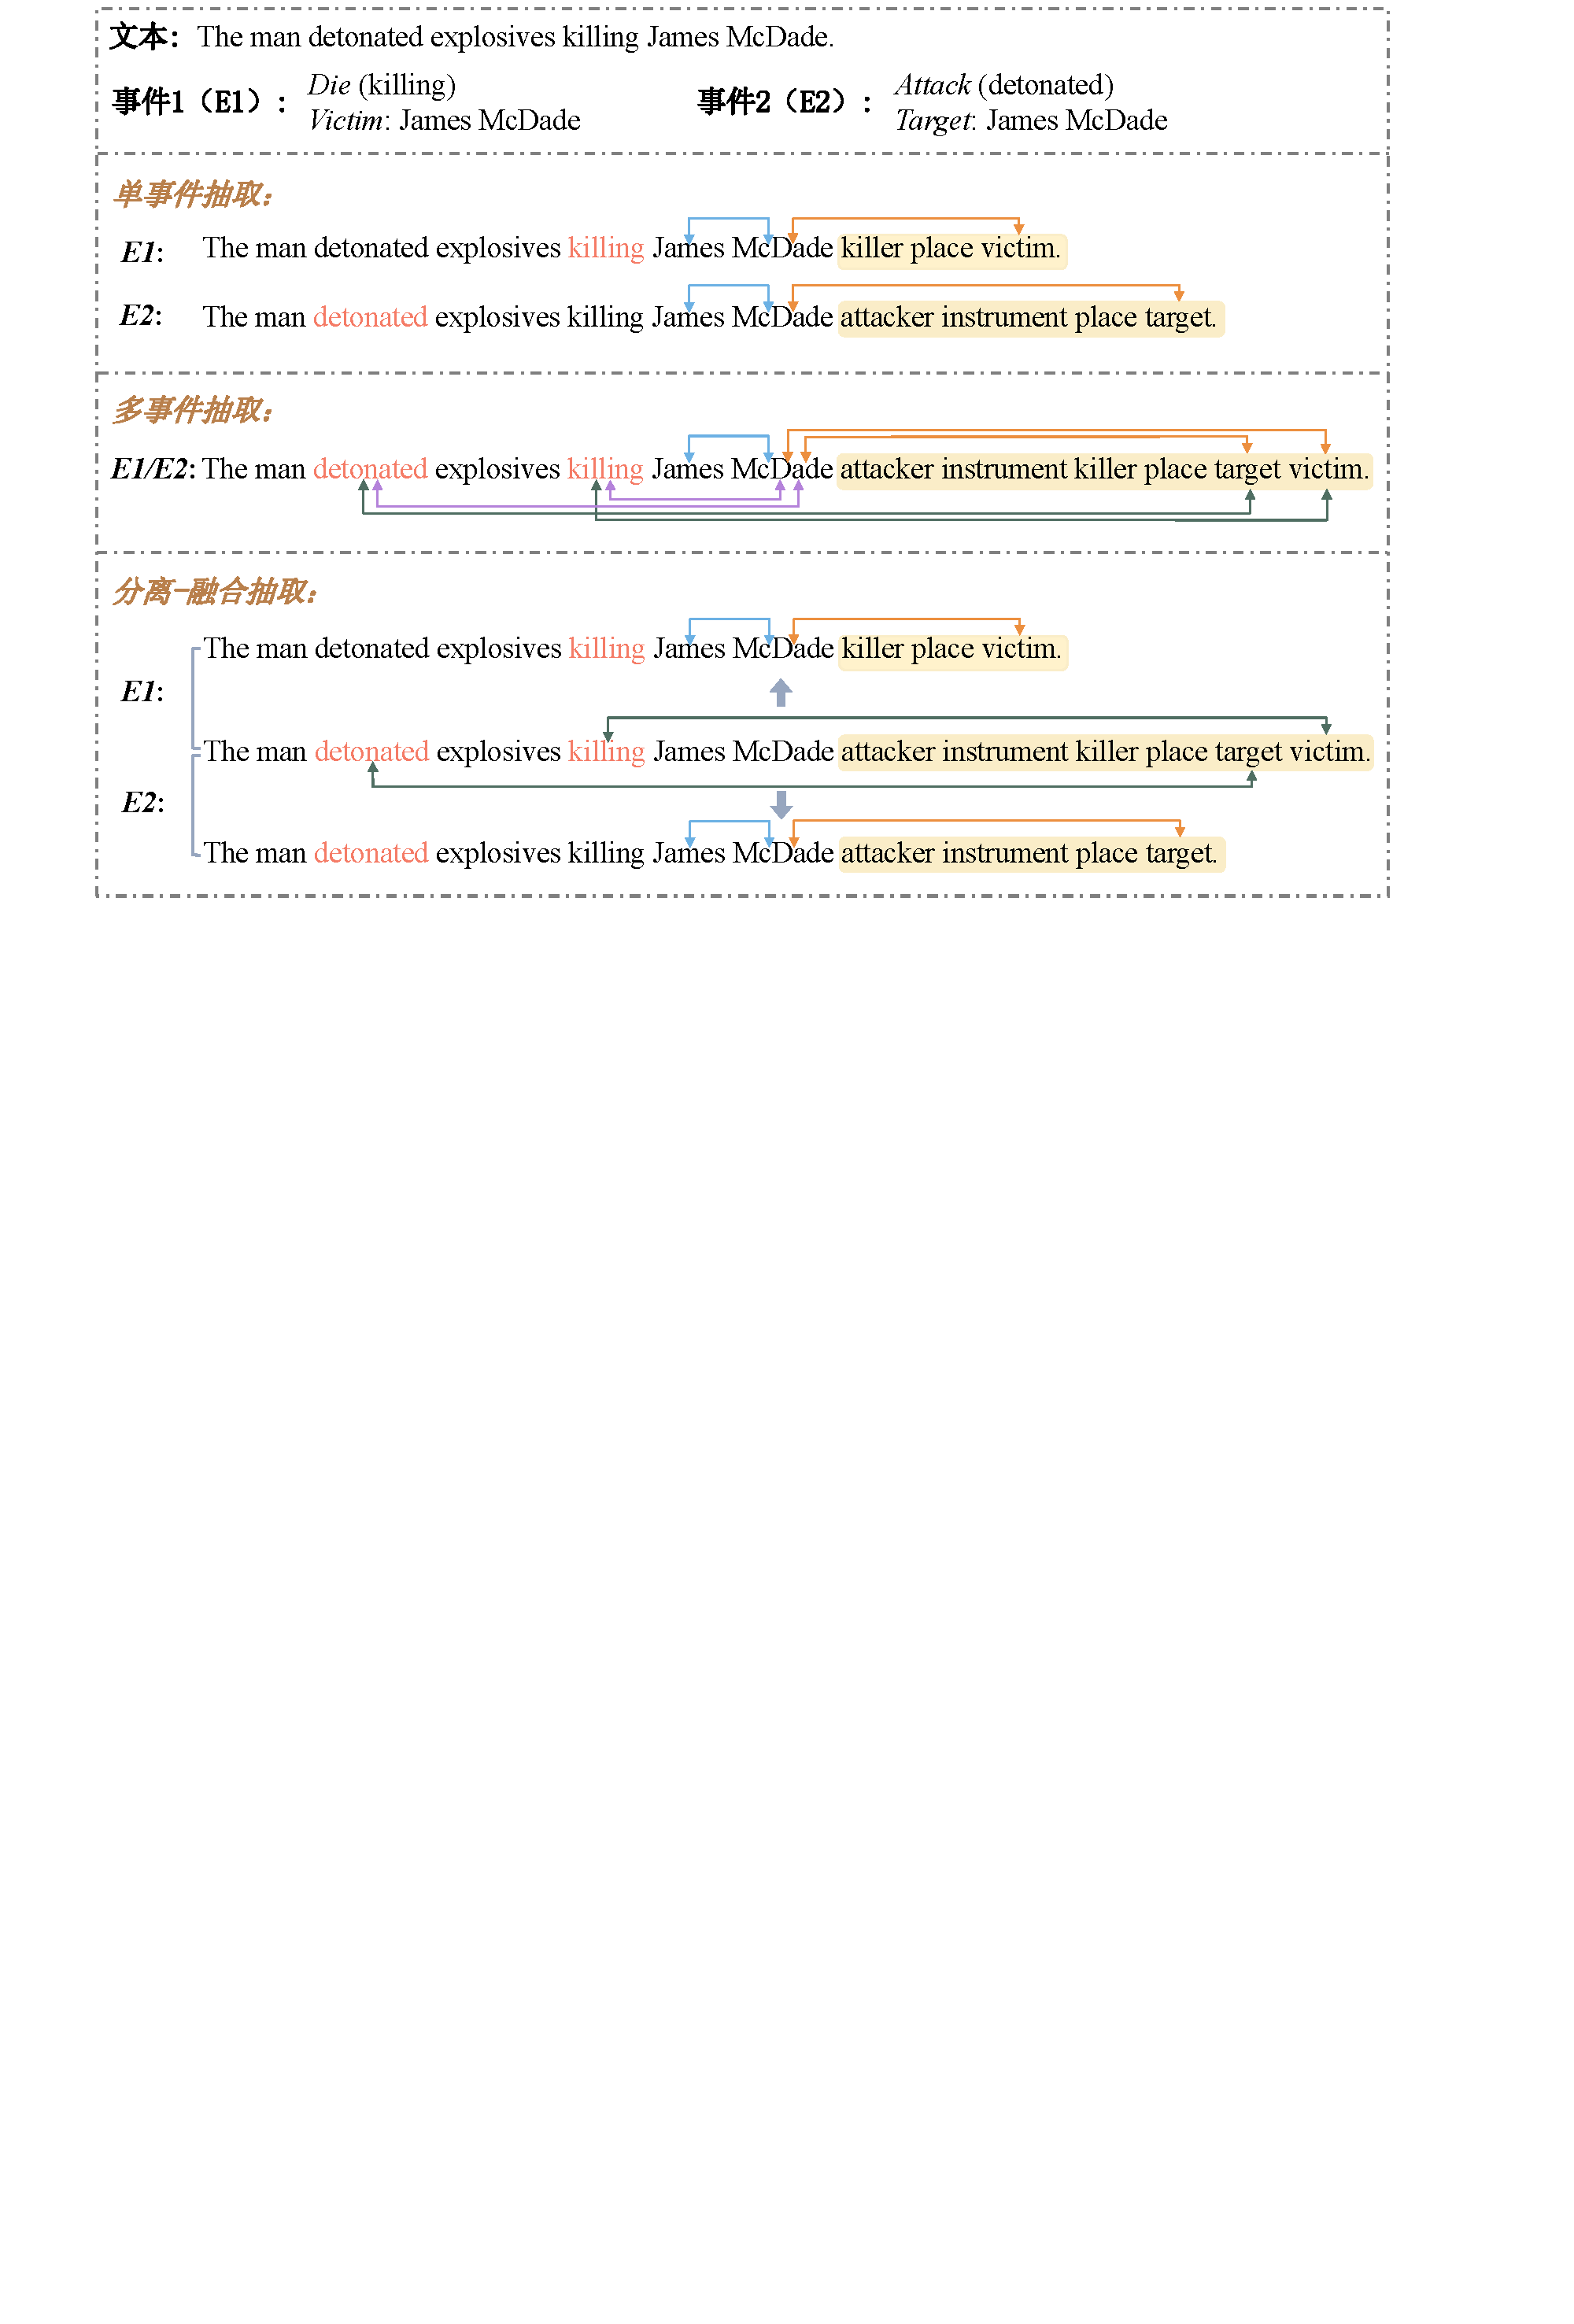
\includegraphics[width=1\columnwidth]{figures/chap5/introduction.pdf} 
\caption{基于不同建模方式的多词元链接事件要素抽取示意图}
% \emph{E1}: \emph{Event 1}. \emph{E2}: \emph{Event 2}. The trigger words are highlighted in red, the concatenated roles are in yellow, and the arrows of different colors represent different linking operations. Note that we only exhibit one argument of each event for simplification.}
\label{example}
\end{figure}

因此,第二种方式的研究~\cite{lou2023universal}一次性抽取多个事件的事件要素。然而,两个新的问题随之而来。首先,与输入文本串接的不再是只在单个事件中出现的要素类型,而是在所有事件中出现的要素类型,这使得通过链接预测选择出正确的要素类型变得更加困难。其次,与单事件抽取方式相比,其需要两种额外的链接操作来确定抽取的事件要素文段和对应的要素类型归属的事件触发词,导致预测阶段积累更多的错误。图\ref{example}展示了同时从$Die$事件和$Attack$事件中抽取事件要素“James McDade”时,其额外增加的触发词-要素文段和触发词-要素类型链接操作。

为了利用上述两种抽取方式的优点,本章设计了一种基于分离-融合范式的跨事件信息构建与利用方法,其先分离跨事件信息获取和事件要素抽取的过程,然后将获取的跨事件信息融合到最终的事件要素抽取中。通过这种分离-融合范式,最终的事件要素抽取可以同时保留单事件抽取方式的简单链接预测和多事件抽取方式的跨事件依赖关系建模能力。图\ref{example}说明了这一范式,其中中间部分从事件要素抽取过程中分离出来,通过触发词-要素类型链接获取跨事件信息,向上和向下的箭头表示跨事件信息的融合。

遵循设计的范式,本章提出了一种新颖的多词元链接事件要素抽取模型去获取分离的跨事件信息并进一步两阶段地融合到最终的事件要素预测(\textbf{Sep}arate acquisition of cross-event information and \textbf{Two}-fold \textbf{F}usion,Sep2F)。为了分离跨事件信息获取和事件要素抽取过程,本章设计了两个多词元链接模块。具体来说,针对多事件中的每个事件,引入一个链接模块来连接事件触发词和其中出现的要素类型。因此,不同事件触发词的特征表示并行聚合了在各自事件中出现的所有要素类型,提供了关键的跨事件信息。同时,引入另一个链接模块抽取目标事件的事件要素。其利用两种链接操作获取事件要素的文段范围和对应的要素类型。在此基础上,本章提出了一个两阶段融合模块将获取的跨事件信息融合到目标事件的要素抽取中。具体地,其首先动态融合来自上述两个链接模块的文本特征表示。然后,利用融合的文本特征表示获取跨模块词元链接分数。该链接分数被进一步融合到最终的预测中。这两阶段的融合过程相互影响,提供了显著的性能贡献。本章的主要贡献可以概括如下:

\begin{itemize}
\item 提出了一种新的基于分离-融合范式的跨事件信息构建与利用方法,其能够同时建模跨事件依赖信息和保留单事件抽取方式的优点。
\item 基于分离-融合范式,提出了一种新的多词元链接事件要素抽取模型,其避免了当前通用事件要素抽取方法的各自局限,且实现了从不同级别文本中通用高效地利用跨事件信息。具体地,设计了两个链接模块,以分别获取跨事件信息和抽取目标事件的事件要素。此外,引入了一个两阶段融合模块,以确保在要素抽取过程中充分利用到获取的跨事件信息。
\item 在四个不同文本级别的数据集上进行了充分的实验,实验结果表明本章所提的模型均显著超越目前性能最优的事件要素抽取基线方法。
\end{itemize}

\section{方法设计}

本章使用$(X,T,C)$表示每个数据实例,其中$X$是输入文本,$T$是目标事件,$C$表示在文本$X$中除目标事件$T$以外的其他事件。具体地,$T$进一步表示为 $\left(e,t,\mathcal{R}^{e}\right)$,其中$e$是事件类型,$t$是事件触发词,$\mathcal{R}^{e}$为只在事件$e$中出现的要素类型集合。类似地,$C$可表示为
$\{(\tilde{e}_i,\tilde{t}_i,\mathcal{R}^{\tilde{e}_i})|~i \leq |C|\}$,其为目标事件$T$提供了跨事件信息。基于此,本章所提模型旨在抽取目标事件$T$的要素集合$\mathcal{A}$,其集合$\mathcal{A}$中的每个事件要素$a^{(r)}$表示要素类型为$r \in \mathcal{R}^{e}$的$X$中文本片段。

如图\ref{framework-sep2f}所示,本章提出的模型由三个模块组成:多事件链接构造、目标事件链接构造和两阶段融合,其遵循了本章设计的分离-融合范式。具体地,前两个模块将跨事件信息的获取和目标事件的要素抽取过程分离,最后一个模块实现了获取的跨事件信息的融合。接下来,本章将具体介绍各个模块。

\begin{figure*}[htp]
\centering
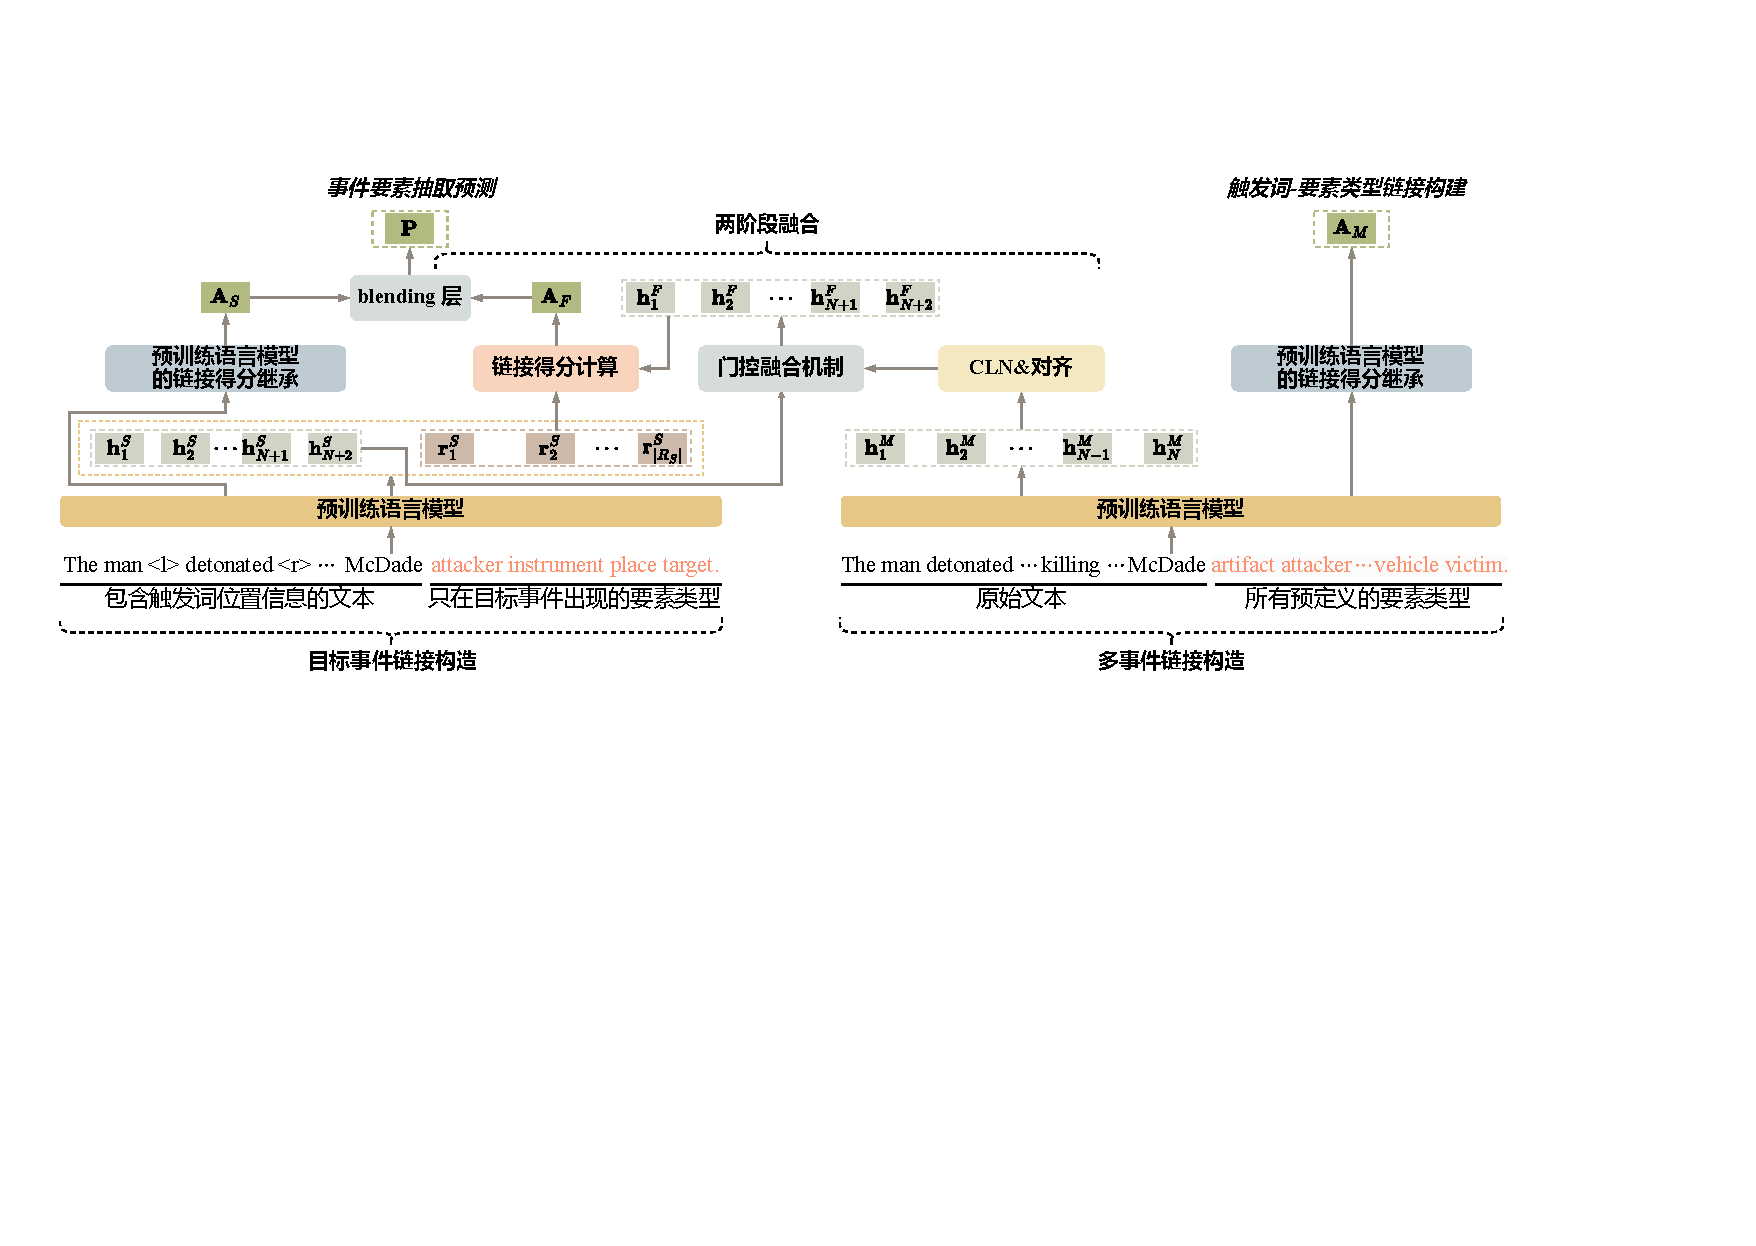
\includegraphics[width=1\linewidth]{figures/chap5/framework.pdf}
\caption{Sep2F模型架构图}
\label{framework-sep2f}
\end{figure*}

\subsection{多事件链接构造}
本模块通过聚合多事件的要素类型信息来获取跨事件信息,其中多事件包含目标事件$T$和所有其他事件$C$。为了实现这种信息聚合,本模块并行地建立不同的事件触发词和它们对应的事件要素类型之间的链接。首先,联合编码待抽取文本和给定数据集中预定义的所有要素类型。然后,根据事件中的触发词-要素类型链接引入标签矩阵和得分矩阵。最后,给出相应的训练损失。

\textbf{编码}~首先,本章利用对应的事件要素名称描述每个事件要素类型,即单个自然语言描述的词。对于名称中包含多个词的少数要素类型,本模型在训练过程中学习额外的特殊词元进行表示。然后,拼接给定数据集中预定义的所有要素类型的名称描述,记作$R_{M}$。在此之后,使用预训练语言模型(PLM)对序列$R_{M}$和输入文本$X$进行联合编码如下:
\begin{equation}
\boldsymbol{E}^{M} = (\boldsymbol{h}_{1}^{M}, \cdots, \boldsymbol{h}_{N}^{M}, \boldsymbol{r}_{1}^{M}, \cdots, \boldsymbol{r}_{|R_{M}|}^{M}) =\textrm{PLM}(X \oplus R_{M})
\end{equation}
其中$\boldsymbol{h}_{n}^{M} \left(1 \leq n \leq N\right)$和 $\boldsymbol{r}_{n}^{M} \left(1 \leq n \leq |R_{M}|\right)$分别为输入文本$X$和事件要素序列$R_{M}$中的词元向量。

\textbf{标签矩阵}~为了学习到多事件各自的要素类型信息,本模块设计了标签矩阵$\boldsymbol{L}_{M} \in {\mathbb{B}}^{(N+|R_{M}|) \times (N+|R_{M}|)}$。对于$T$或$C$中的每个事件,假设其触发词的开始和结束词元向量分别是
$\boldsymbol{h}_{i}^{M}$和$\boldsymbol{h}_{j}^{M}$。进一步,对于该事件中出现的每个要素类型,假设其对应的词元向量是$\boldsymbol{r}_{k}^{M}$。然后,实施链接操作来连接触发词和该要素类型。具体来说,分别构造链接词元对$(i,k+N)$和 $(k+N,j)$,并相应地设置${L}_{M}[i][k+N]$和${L}_{M}[k+N][j]$为“\emph{True}”。对于没有链接的词元对,本模块将$\boldsymbol{L}_{M}$中的相应值标记为“\emph{False}”。图\ref{multi_event_label}展示了$\boldsymbol{L}_{M}$的一个示例,其中被红色标记的为事件触发词词元,被黄色标记的为所有预定义的事件要素类型词元,“\textbf{-}”表示“\emph{False}”。根据图\ref{multi_event_label}可知,“detonated”触发的事件中存在要素类型$Target$,而“killing”触发的事件中存在要素类型$Victim$。

\begin{figure}[htp]
\centering
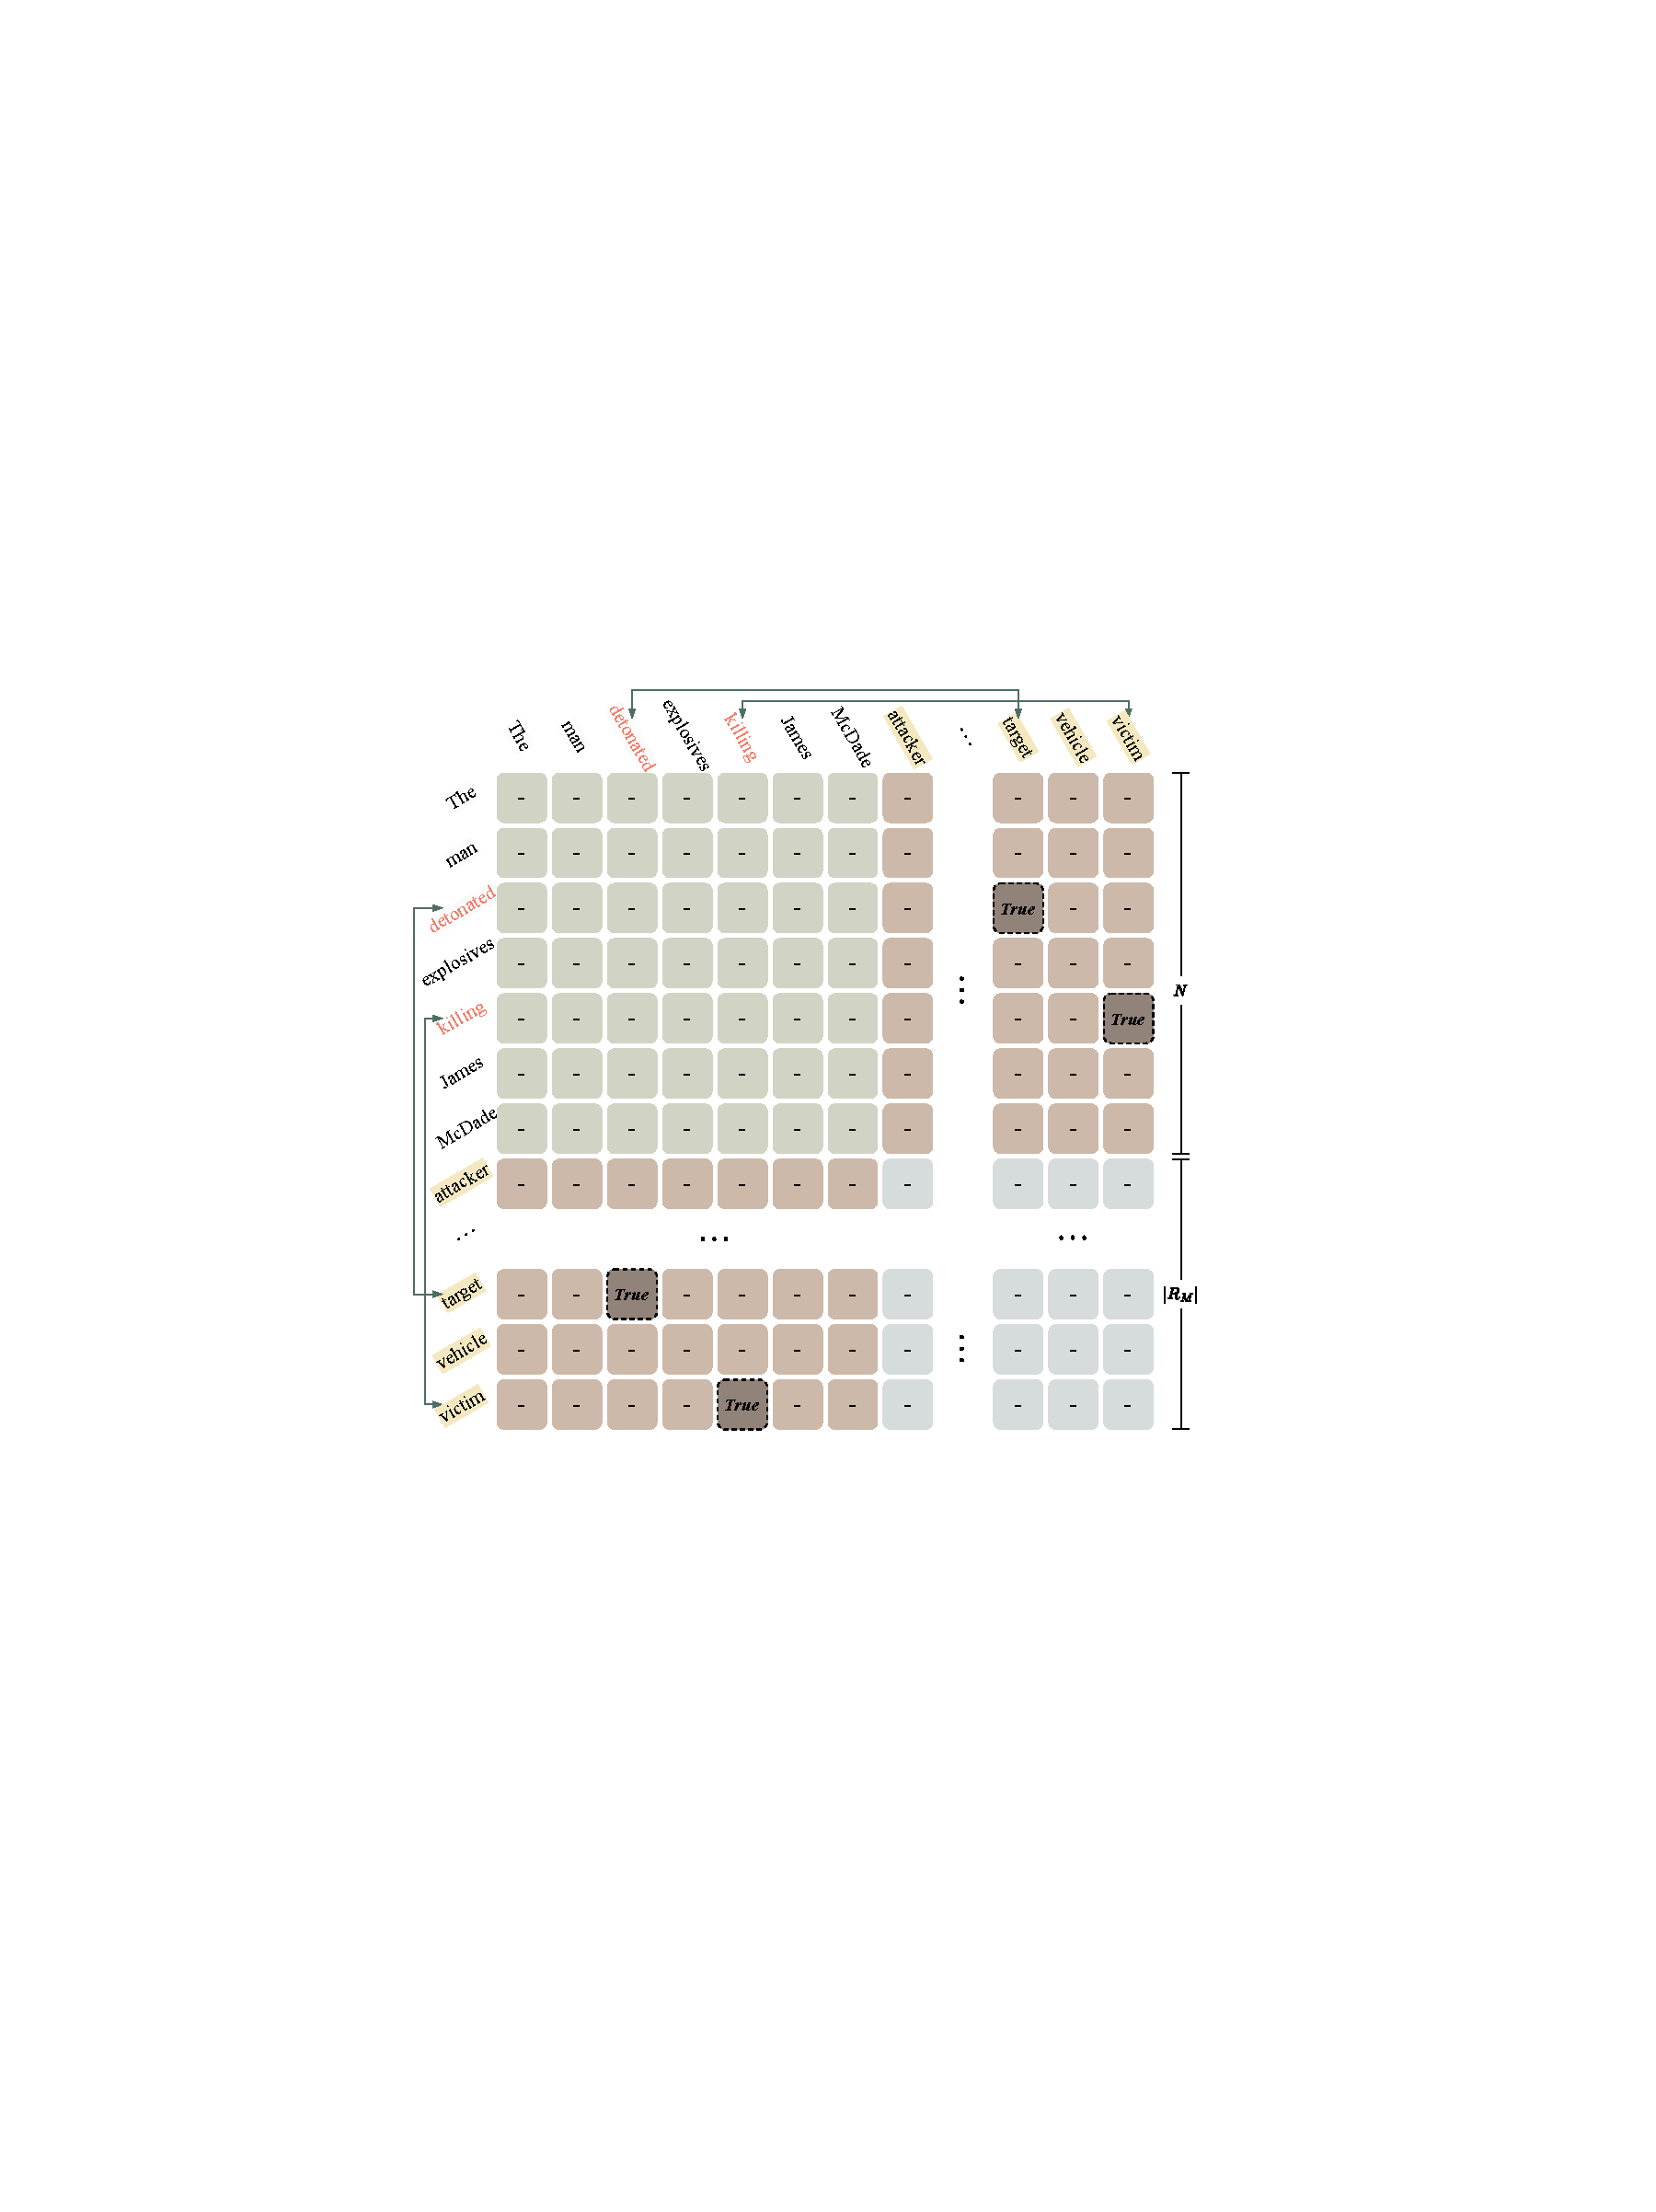
\includegraphics[width=0.6\linewidth]{figures/chap5/label_multi_frame.pdf}
\caption{标签矩阵$\boldsymbol{L}_{M}$示例图}
\label{multi_event_label}
\end{figure}

\textbf{得分矩阵}~受Tang等人~\cite{tang2022unirel}研究工作的启发,本模块继承基于Transformer架构的预训练语言模型的多头自注意力结果作为不同词元对之间的链接分数。具体来说,根据选定的预训练语言模型的最后一层,获取其未经过softmax归一化的多头自注意力权重,并进行均值计算:
\begin{equation}
\boldsymbol{A}_{M}=\frac{1}{P} \sum_p^P \frac{\boldsymbol{Q}_{p} \boldsymbol{K}_{p}^\top}{\sqrt{d_h}}
\label{scores}
\end{equation}
其中$P$为多头的数目,$d_h$为多头自注意机制中查询向量和键向量的维度,$\boldsymbol{Q}_{p}$和$\boldsymbol{K}_{p}$分别为查询矩阵和键矩阵,$\boldsymbol{A}_{M} \in {\mathbb{R}}^{(N+|R_{M}|) \times (N+|R_{M}|)}$表示多事件的触发词-要素类型链接得分。

\textbf{训练损失}~本模块使用训练损失$\mathcal{L_\textrm{TR}}$去指导模型学习不同事件触发词及其相应出现的要素类型之间的链接,如下所示:

\begin{equation}
\begin{split}
    \mathcal{L_\textrm{TR}} = & -\frac{1}{(N+|R_{M}|)^2} \sum_i \sum_j\left(L^{M}_{i,j} \log \sigma\left({A}_{M}[i][j]\right) + \right. \\
    & \left. (1-L^{M}_{i,j}) \log \left(1-\sigma\left({A}_{M}[i][j]\right)\right) \right)
\end{split}
\end{equation}
其中$\sigma(\cdot)$为sigmoid激活函数。当${L}_{M}[i][j]$为“\emph{True}”时,设置$L^{M}_{i,j}$为1,否则设置$L^{M}_{i,j}$为0。

\subsection{目标事件链接构造}
\label{target_event_module}
为了抽取给定目标事件$\left(e,t,\mathcal{R}^{e}\right)$的事件要素,本模块对输入文本和只在事件$e$中出现的要素类型进行联合编码,然后定义对应的多词元链接标签矩阵和得分矩阵,并给出相应的训练损失计算。

\textbf{编码}~与多事件链接构造模块不同,本模块拼接所有$\mathcal{R}^{e}$集合中的事件要素类型的名称描述,记作$R_{S}$。然后,遵循Ma等人~\cite{ma2022prompt}的研究工作在文本$X$中插入两个特殊词元$\langle \ell \rangle$和 $\langle r \rangle$,以便标记触发词$t$的位置:
\begin{equation}
X_{S}=(x_{1},\cdots,\langle \ell \rangle,t,\langle r \rangle,\cdots, x_{|X|})
\end{equation}
在此之后,将包含触发词位置信息的文本$X_{S}$和要素类型序列$R_{S}$进行串接,并利用另一个预训练语言模型对其进行编码:
\begin{equation}
\boldsymbol{E}^{S} = (\boldsymbol{h}_{1}^{S}, \cdots, \boldsymbol{h}_{N+2}^{S}, \boldsymbol{r}_{1}^{S}, \cdots, \boldsymbol{r}_{|R_{S}|}^{S}) =\textrm{PLM}(X_{S} \oplus R_{S})
\end{equation} 
其中$\boldsymbol{h}_{n}^{S} \left(1 \leq n \leq N+2\right)$和$\boldsymbol{r}_{n}^{S} \left(1 \leq n \leq |R_{S}|\right)$分别为$X_{S}$和$R_{S}$中的词元向量。

\textbf{标签矩阵}~为了标记给定目标事件中的事件要素文段范围和要素类型,本模块定义了标签矩阵$\boldsymbol{L}_{S} \in {\mathbb{B}}^{(N+|R_{S}|+2) \times (N+|R_{S}|+2)}$。对于目标事件中的每个事件要素,假设其文段的开始和结束词元向量分别是$\boldsymbol{h}_{i}^{S}$和 $\boldsymbol{h}_{j}^{S}$,其要素类型对应的词元向量是$\boldsymbol{r}_{k}^{S}$。基于此,首先构造链接词元对$(i,j)$和$(j,i)$并设置${L}_{S}[i][j]$和${L}_{S}[j][i]$为“\emph{True}”,以用来标记事件要素的文段。同时,通过要素文段-要素类型链接操作来标记事件要素对应的要素类型信息。相应地,构造两个链接对$(i,k+N+2)$和$(k+N+2,j)$,并设置${L}_{S}[i][k+N+2]$和${L}_{S}[k+N+2][j]$为“\emph{True}”。对于没有链接的词元对,将$\boldsymbol{L}_{S}$中的相应值设置为“\emph{False}”。图\ref{single_event_label}展示了$\boldsymbol{L}_{S}$的一个示例,其中被红色标记的为事件触发词词元,被黄色标记的为只在该事件触发词对应的事件类型中出现的事件要素类型词元,“\textbf{-}”表示“\emph{False}”。根据图\ref{single_event_label}可知,在“detonated”触发的事件中,存在事件要素“James McDade”,其对应的要素类型为$Target$。

\begin{figure}[htp]
\centering
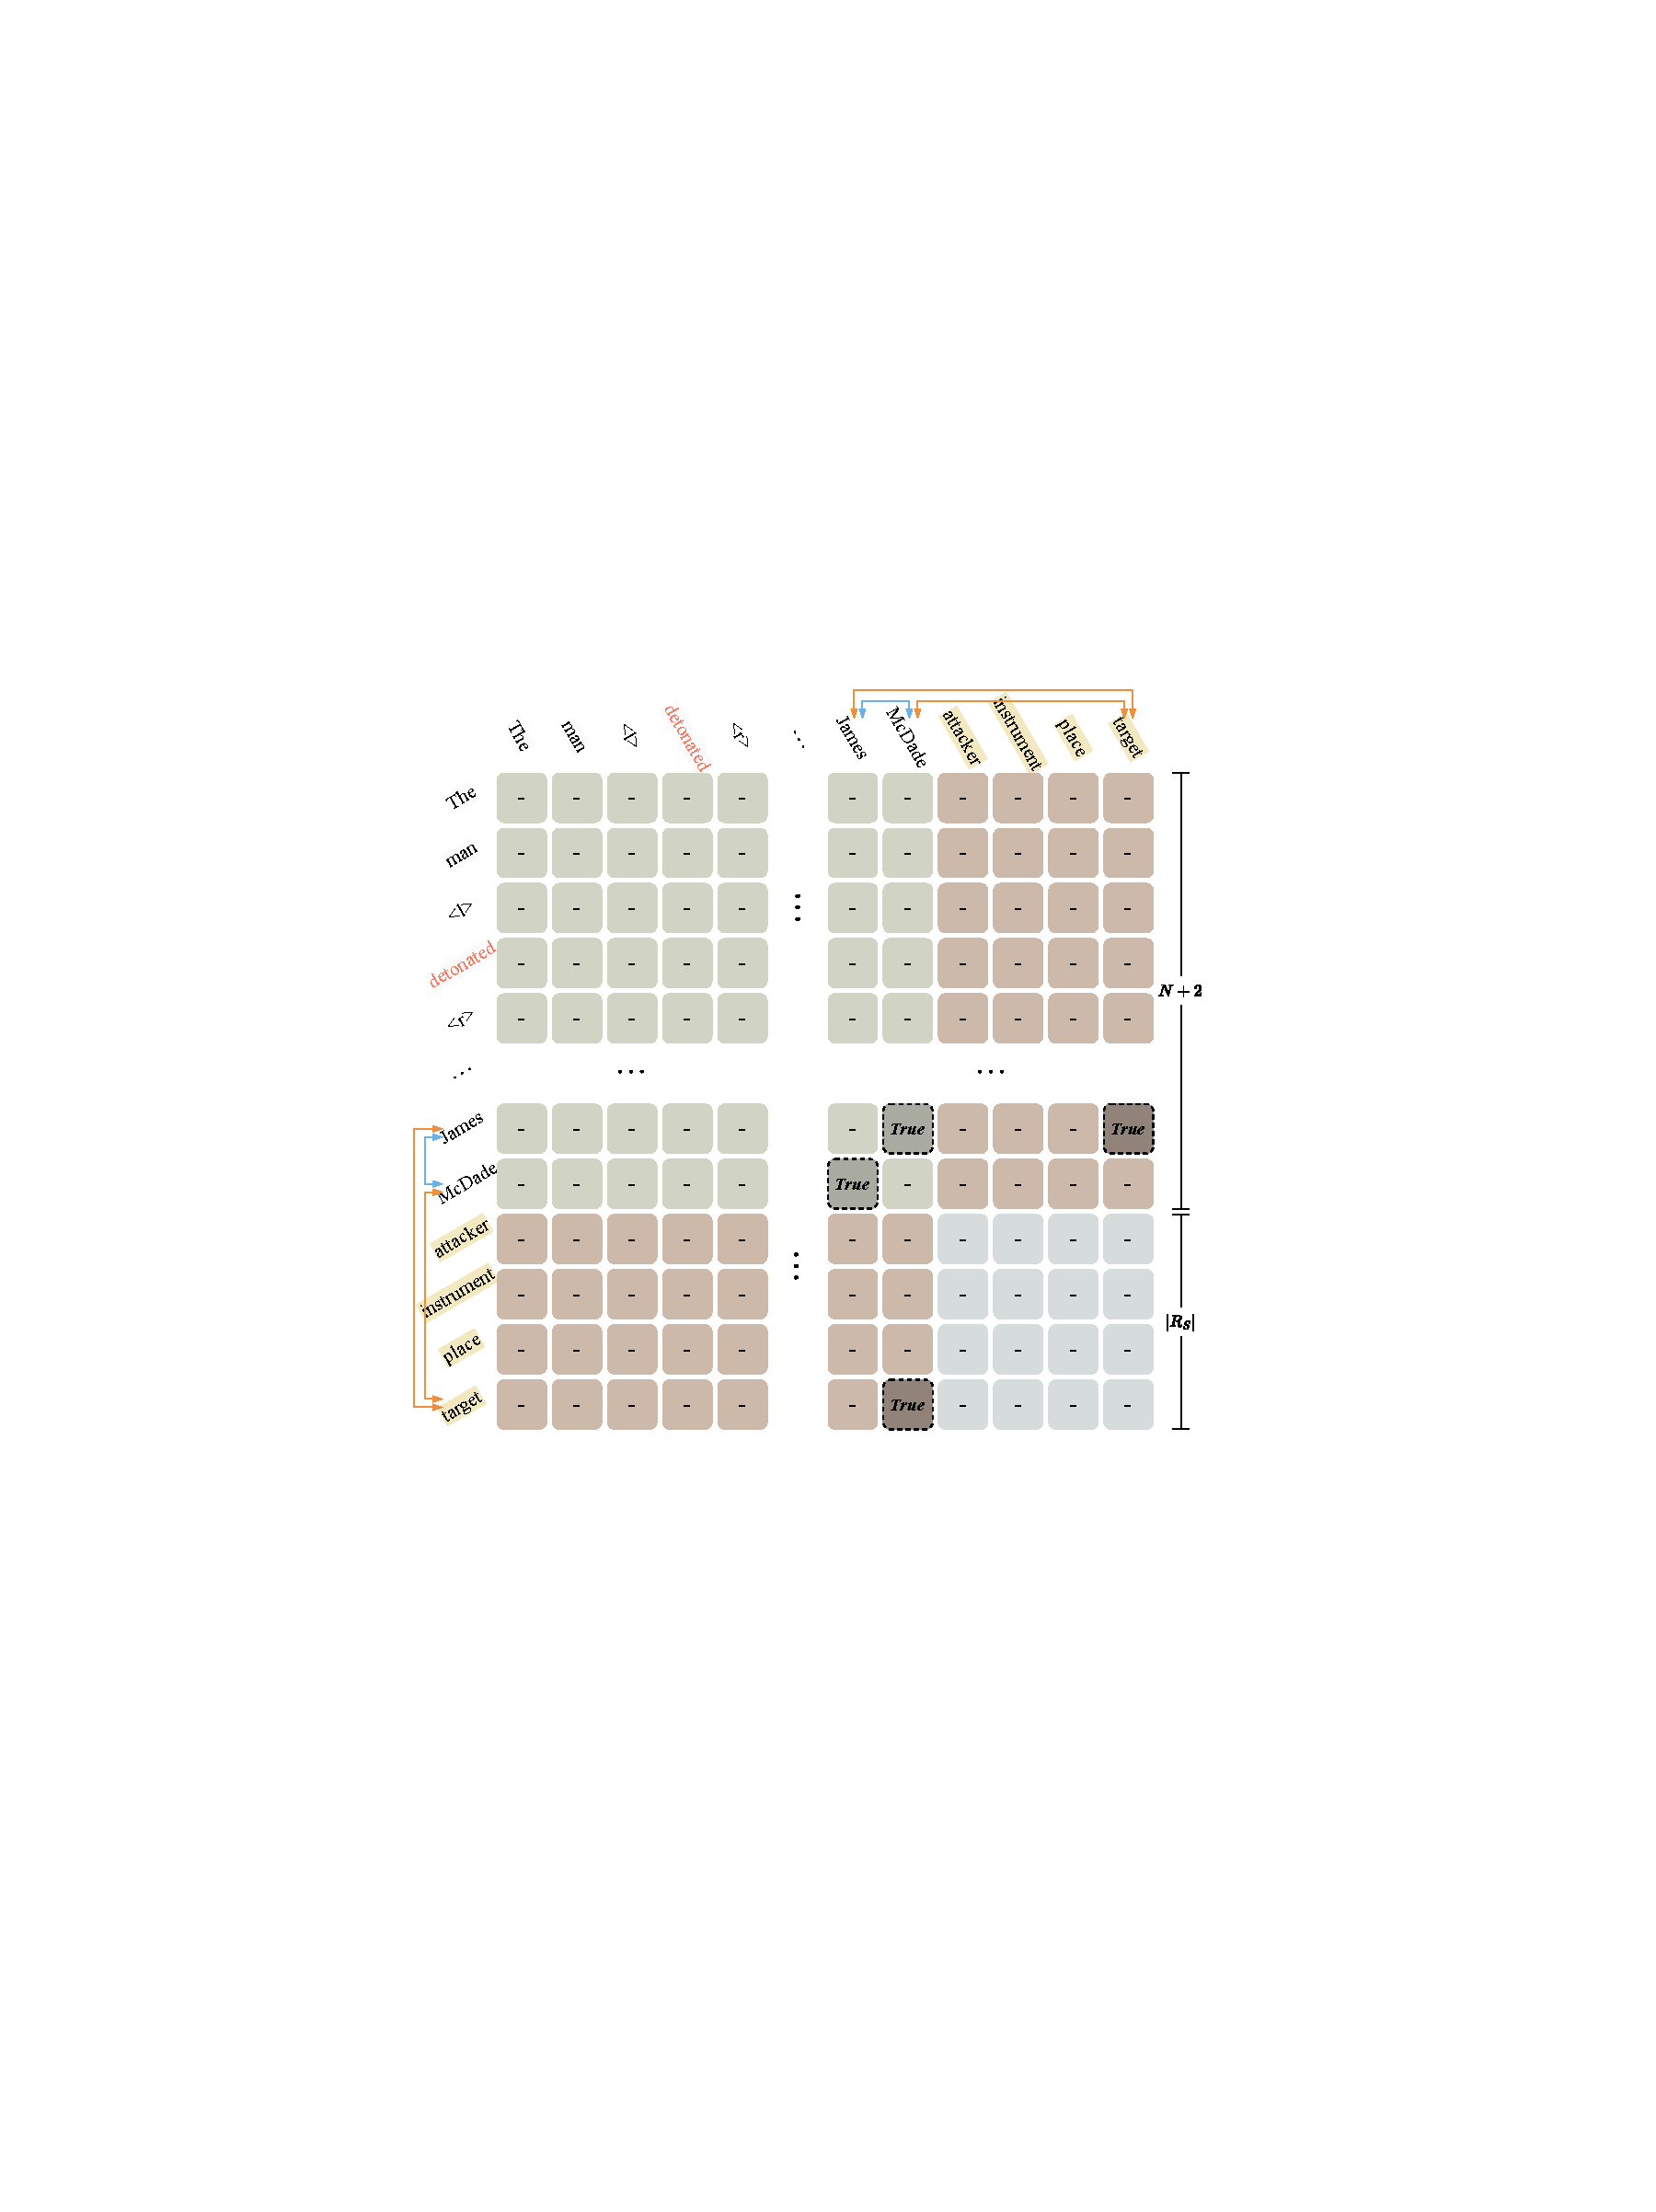
\includegraphics[width=0.6\linewidth]{figures/chap5/label_single_frame.pdf}
\caption{标签矩阵$\boldsymbol{L}_{S}$示例图}
\label{single_event_label}
\end{figure}

\textbf{得分矩阵}~与多事件链接构造模块中的公式\ref{scores}相同,本模块同样根据所使用的预训练语言模型的最后一层,利用其未通过softmax归一化的平均多头自注意权重作为多词元间的链接分数,表示为$\boldsymbol{A}_{S} \in {\mathbb{R}}^{(N+|R_{S}|+2) \times (N+|R_{S}|+2)}$。

\textbf{训练损失}~为了利用到获取的跨事件信息,首先采用两阶段融合模块(其将在下一模块中作详细介绍)来得到最终的词元链接预测矩阵:
\begin{equation}
\boldsymbol{P} =\textrm{TFF}(\boldsymbol{E}^{M},\boldsymbol{E}^{S},\boldsymbol{A}_{S})
\end{equation} 
其中$\textrm{TFF}$指两阶段融合模块。然后,可以得到训练损失$\mathcal{L_\textrm{EAE}}$如下:\begin{equation}
\label{binary}
\begin{split}
    \mathcal{L_\textrm{EAE}} = & -\frac{1}{(N+|R_{S}|+2)^2} \sum_i \sum_j\left(L^{S}_{i,j} \log {P}[i][j] + \right. \\
    & \left. (1-L^{S}_{i,j}) \log \left(1- {P}[i][j]\right) \right)
\end{split}
\end{equation} 
其中当${L}_{S}[i][j]$为“\emph{True}”时,设置
$L^{S}_{i,j}$为1,否则设置$L^{S}_{i,j}$为0。

\subsection{两阶段融合}
\label{two-fold}
本模块利用聚合了跨事件要素类型信息的文本表示来增强目标事件的要素抽取。具体地,首先动态融合来自上述两个链接模块的文本表示,即第一阶段融合。然后,使用融合的文本表示来获得目标事件的另一个词元链接得分矩阵,其不同于$\boldsymbol{A}_{S}$。这两个词元链接得分矩阵进一步被融合为最终的链接预测,即第二阶段融合。

\textbf{第一阶段融合}~由于$\boldsymbol{E}^{M}$中的文本向量涉及多事件信息,本模块首先利用条件层归一化(Conditional Layer Normalization,CLN)~\cite{yu2021semi,xu2022extracting}来获取与目标事件(触发词)相关的上下文向量。对于目标事件触发词$t$,本模块简单地将其输入到一个参数冻结的预训练语言模型中,并使用得到的第一个词元向量来表示该触发词,记作$\boldsymbol{t}$。然后,对于$\boldsymbol{E}^{M}$中的每个词元向量$\boldsymbol{h}_{n}^{M} \left(1 \leq n \leq N\right)$,可得到相应的向量$\boldsymbol{\hat{h}}_{n}^{M} \left(1 \leq n \leq N\right)$如下:
\begin{equation}
    \boldsymbol{\alpha}_{t}=\boldsymbol{t}\boldsymbol{W}_\alpha+\boldsymbol{b}_\alpha
\end{equation}
\begin{equation}
    \boldsymbol{\beta}_{t}=\boldsymbol{t}\boldsymbol{W}_\beta+\boldsymbol{b}_\beta
\end{equation}
\begin{equation}
    \boldsymbol{\hat{h}}_{n}^{M} = \textrm{CLN}(\boldsymbol{h}_{n}^{M}, \boldsymbol{\alpha}_{t}, \boldsymbol{\beta}_{t})=\boldsymbol{\alpha}_{t} \odot\left(\frac{\boldsymbol{h}_{n}^{M}-\mu}{\sigma}\right)+\boldsymbol{\beta}_{t}
\end{equation}
其中$\boldsymbol{W}_\alpha \in {\mathbb{R}}^{d_{1} \times d_{1}}$, $\boldsymbol{W}_\beta \in {\mathbb{R}}^{d_{1} \times d_{1}}$, $\boldsymbol{b}_\alpha \in {\mathbb{R}}^{d_{1}}$和$\boldsymbol{b}_\beta \in {\mathbb{R}}^{d_{1}}$为可训练的参数,$\mu$和$\sigma$分别为根据$\boldsymbol{h}_{n}^{M}$中的向量元素计算得到的平均值和标准偏差,$d_{1}$为向量$\boldsymbol{t}$的维度。然后,在$(\boldsymbol{\hat{h}}_{1}^{M}, \cdots, \boldsymbol{\hat{h}}_{N}^{M})$中插入零向量$\boldsymbol{0}$,以便与文本向量$\boldsymbol{E}^{S}$进行对齐:
\begin{equation}
(\boldsymbol{\bar{h}}_{1}^{M}, \cdots, \boldsymbol{\bar{h}}_{N+2}^{M}) = (\boldsymbol{\hat{h}}_{1}^{M}, \cdots, \boldsymbol{0}, \boldsymbol{\hat{h}}_{i}^{M}, \cdots, \boldsymbol{\hat{h}}_{j}^{M}, \boldsymbol{0}, \cdots, \boldsymbol{\hat{h}}_{N}^{M})
\end{equation} 
其中$i$和$j$对应于触发词$t$的词元向量在$(\boldsymbol{h}_{1}^{S}, \cdots, \boldsymbol{h}_{N+2}^{S})$中的开始和结束位置。最后,动态融合不同的文本向量。给定两个词元向量 $\boldsymbol{h}_{n}^{S}$和$\boldsymbol{\bar{h}}_{n}^{M}$ $(1 \leq n \leq N+2)$,本模块使用门控融合机制以获取词元向量$\boldsymbol{h}_{n}^{F}$:
\begin{equation}
\boldsymbol{g}_{n}=\sigma\left(\left[\boldsymbol{h}_{n}^{S}; \boldsymbol{\bar{h}}_{n}^{M}\right]\boldsymbol{W}_{G}\right)
\end{equation} 
\begin{equation}
\boldsymbol{h}_{n}^{F} = \boldsymbol{g}_{n} \odot \boldsymbol{h}_{n}^{S} + \left(1-\boldsymbol{g}_{n}\right) \odot \boldsymbol{\bar{h}}_{n}^{M}
\end{equation} 
其中$\sigma(\cdot)$为sigmoid函数,$\boldsymbol{W}_{G} \in {\mathbb{R}}^{2d_{1} \times d_{1}}$为可训练学习的矩阵,$\odot$表示元素依次相乘操作。

\textbf{第二阶段融合}~首先,串接融合的文本向量$(\boldsymbol{h}_{1}^{F}, \cdots, \boldsymbol{h}_{N+2}^{F})$和要素类型对应的词元向量$(\boldsymbol{r}_{1}^{S}, \cdots, \boldsymbol{r}_{|R_{S}|}^{S})$,表示为$\boldsymbol{F}$。然后,本模块计算另一个词元链接得分矩阵$\boldsymbol{A}_{F} \in {\mathbb{R}}^{(N+|R_{S}|+2) \times (N+|R_{S}|+2)}$如下:
\begin{equation}
\boldsymbol{F}_{Q}=\boldsymbol{F} \boldsymbol{W}_{Q},~\boldsymbol{F}_{K}=\boldsymbol{F} \boldsymbol{W}_{K}
\end{equation} 
\begin{equation}
    \boldsymbol{A}_{F}=\boldsymbol{F}_{Q} \boldsymbol{F}_{K}^\top
\end{equation}
其中$\boldsymbol{W}_{Q} \in {\mathbb{R}}^{d_{1} \times d_{2}}$和$\boldsymbol{W}_{K} \in {\mathbb{R}}^{d_{1} \times d_{2}}$为可训练学习的矩阵。最后,根据$\boldsymbol{A}_{F}$和章节\ref{target_event_module}中得到的得分矩阵$\boldsymbol{A}_{S}$,使用blending层~\cite{wolpert1992stacked}融合如下:
\begin{equation}
\boldsymbol{P}=\sigma (\boldsymbol{A}_{S} + \boldsymbol{A}_{F} - \tau)
\end{equation} 
其中$\tau$为可训练的参数。

\subsection{训练和推理}
\textbf{训练}~本章提出模型的整体训练损失可根据如下得到:  
\begin{equation}
 \mathcal{L} = \alpha \mathcal{L_\textrm{EAE}} + (1-\alpha) \mathcal{L_\textrm{TR}}
 \label{overall_loss}
\end{equation}
其中$\alpha\,(0 < \alpha < 1)$为权重参数。

\textbf{推理}~基于词元链接预测矩阵$\boldsymbol{P}$,对于其中的每一个链接对$(i,j)$,如果对应预测值${P}[i][j](1 \leq i,j \leq N+|R_{S}|+2)$超过设定的阈值参数$\delta$,则将该链接对添加到链接对集合$\mathcal{C}$中。然后,使用$\mathcal{C}$作为输入,运行如算法\ref{algorithm_arg}所示的推理算法,得到目标事件的要素集合$\mathcal{A}$。对于$\mathcal{A}$中的每个元素$(start, end, role)$,$start$和$end$分别表示要素的开始和结束位置,$role$为对应的要素类型在$R_{S}$中的索引。 

\begin{algorithm}[tb]
\caption{目标事件的要素推理}
\label{algorithm_arg}
\textbf{Input}: 预测的链接对集合$\mathcal{C}((s_{k},e_{k})), k \in (1,\cdots,|\mathcal{C}|)$.\\
\textbf{Output}: 事件要素集合$\mathcal{A}$.
\begin{algorithmic}[1] %[1] enables line numbers
\STATE $cand\_span=set()$.
\STATE $start2r\_dict=\{\}$,~$end2r\_dict=\{\}$.
\FOR{$(s_{k}, e_{k}) \in \mathcal{C}$}
\IF {$s_{k} \leq N+2$ \AND $e_{k} \leq N+2$}
\STATE 将元组$(s_{k},e_{k})$添加到集合$cand\_span$
\ELSIF{$s_{k} \leq N+2$ \AND $e_{k} > N+2$}
\STATE 将键值对$(s_{k},e_{k}-N-2)$添加到字典$start2r\_dict$
\ELSIF{$s_{k} > N+2$ \AND $e_{k} \leq N+2$}
\STATE 将键值对$(e_{k},s_{k}-N-2)$添加到字典
$end2r\_dict$
\ENDIF
\ENDFOR
\FOR{$(s, e) \in cand\_span$}
\FOR{$r \in (\textrm{set}(start2r\_dict[s])~\cap~\textrm{set}(end2r\_dict[e]))$}
\STATE 将元组$(s,e,r)$添加到集合$\mathcal{A}$
\ENDFOR
\FOR{$r \in (\textrm{set}(start2r\_dict[e])~\cap~\textrm{set}(end2r\_dict[s]))$}
\STATE 将元组$(e,s,r)$添加到集合$\mathcal{A}$
\ENDFOR
\ENDFOR
\end{algorithmic}
\end{algorithm}

\section{实验评估}
\label{section_5_3}
\subsection{实验设置}
\textbf{1.数据集}~为了评估所提模型,本章将在以下数据集上进行实验:
\begin{itemize}
\item ACE2005~\cite{doddington2004automatic} - 该数据集详细介绍见章节\ref{experiment_settings}。本章实验使用其事件标注数据进行句子级别事件要素抽取的评估。在数据预处理上,与章节\ref{settings_4}不同,本章遵循PAIE~\cite{ma2022prompt}和TabEAE~\cite{he2023revisiting}等通用事件要素抽取模型的设置,使用Du等人~\cite{du2020event}的预处理脚本。该脚本遵循DyGIE++~\cite{wadden2019entity}模型的设置。

\item RAMS~\cite{ebner2020multi} - 该文档级别事件要素抽取数据集来源于新闻文章。与原始数据集将同一上下文中的多个事件视为不同的实例不同,本章实验遵循TabEAE的预处理过程,聚合每个实例的同一上下文中出现的其他事件的标注信息。

\item WikiEvents~\cite{li2021document} - 该文档级别数据集来源英文维基百科。本章实验遵循PAIE的预处理程序,采用以每个目标事件触发词为中心的预定义窗口去截断过长的上下文内容,避免超出预训练语言模型的输入长度限制。

\item MLEE~\cite{pyysalo2012event} - 该文档级别事件要素抽取数据集基于生物医学领域的英文出版物摘要标注得到。在预处理方面,遵循TabEAE参照Trieu等人~\cite{trieu2020deepeventmine}的预处理设置。此外,由于MLEE数据集中不存在验证集,本章实验遵循TabEAE使用训练集调整模型的超参数。    
\end{itemize}

对于所有文档级别数据集,遵循He等人~\cite{he2023revisiting}设置预定义的窗口长度为250,将每个文档拆分为多个上下文片段。本章实验所用数据集的具体统计数据如表\ref{statistics}所示。

\begin{table}[htp]
\centering
\caption{数据集详细统计信息} 
% \emph{Avg Args} denotes the average number of arguments per event.
\begin{tabular}{l|cccc}
\toprule
 数据集 & ACE2005 & RAMS & WikiEvents & MLEE  \\
 \midrule
 \textbf{\#事件} &  &  &  &  \\
 训练集 & 4,202 & 7,329 & 3,241 & 4,442  \\
 验证集 & 450 & 924 & 345 & -  \\
 测试集 & 403 & 871 & 365 & 2,200  \\
 \midrule
 \textbf{\#事件要素} &  &  &  &  \\
 训练集 & 4,859 & 17,026 & 4,552 & 5,786 \\
 验证集 & 605 & 2,188 & 428 & - \\
 测试集 & 576 & 2,023 & 566  & 2,764 \\
 \midrule
 \textbf{\#事件类型} & 33 & 139 & 50 & 23  \\
 \textbf{\#要素类型} & 22 & 65 & 59 & 8 \\
 % \textbf{\#Avg Args} & 1.19 & 2.33 & 1.40 & 1.29  \\
\bottomrule
\end{tabular}
\label{statistics}
\end{table}

\textbf{2.评价指标}~
遵循之前通用文本级别事件要素抽取研究工作~\cite{ma2022prompt,he2023revisiting},本章采用两个指标来衡量模型性能。(1)要素识别F1得分(Argument Identification F1 score,Arg-I):当其事件要素文段的边界与事件中任意一个标注的要素相匹配,则认为该事件要素被正确识别。基于该识别准则,本章进一步计算对应的F1值评估要素识别性能,其F1值计算参照章节\ref{experiment_settings}。(2)要素分类F1得分(Argument Classification F1 score,Arg-C):当其事件要素文段的边界和要素类型都与事件中任意一个标注的要素相匹配,则认为该事件要素被正确分类。基于该分类准则,本章进一步计算对应的F1值评估要素分类性能,其F1值计算参照章节\ref{experiment_settings}。在实验中,使用三个不同的随机种子训练本章提出的Sep2F模型,并通过平均值计算得到相应的性能结果。

\textbf{3.实验配置}~
% \label{settings}
为了便于与最近的研究工作进行公平比较,本章实验在模型中使用RoBERTa-base和RoBERTa-large~\cite{liu2019roberta}作为预训练语言模型,其分别基于Huggingface上发布的“FacebookAI/roberta-base”文件\footnote{https://huggingface.co/FacebookAI/roberta-base}和“FacebookAI/roberta-large”文件\footnote{https://huggingface.co/FacebookAI/roberta-large}进行参数初始化。基于此两种模型,均采用配备了线性学习率调度器的Adam优化器和比率为0.1的warmup策略。$\delta$为等式\ref{binary}中二分类预测值${P}[i][j]$的推断阈值,因此实验中遵循常规的二分类设置,在所有数据集上均设置$\delta$为0.5。在RAMS数据集上设置训练轮次为50,在其他数据集上设置训练轮次为100。在ACE2005数据集上设置批数据大小为16,在其他数据集上设置批数据大小为8。对于ACE2005,$d_{2}$设置为32,而在其他数据集上$d_{2}$设置为64。此外,基于每个数据集的验证集,使用网格搜索调整各自模型的学习率和训练权重$\alpha$。具体地,在区间$\{0.5,~0.6,~0.7,~0.8,~0.9\}$内调整权重$\alpha$,在区间$\{3,~4,~5\} \times 10^{-5}$和$\{1,~2,~3\} \times 10^{-5}$内分别搜索基于RoBERTa-base和RoBERTa-large的模型的最佳学习率。表\ref{hyperparameter}列出了在不同数据集上最终选择的训练权重和学习率,其中表格上半部分为基于RoBERTa-base的模型的参数详情,表格下半部分为基于RoBERTa-large的模型的参数详情。对于基于RoBERTa-base的模型,不同数据集上的训练均在相同实验服务器上完成,具体配置为:CPU型号Intel(R) Xeon(R) Gold 5320,主频2.20GHz;内存256G;GPU计算卡型号NVIDIA GeForce RTX 3090,显存24G。对于基于RoBERTa-large的模型,其具体配置为:CPU型号Intel(R) Xeon(R) Silver 4314,主频2.40GHz;内存128G;GPU计算卡型号NVIDIA A100 PCIE,显存40G。本章实验均基于Pytorch~\cite{paszke2017automatic}框架完成。

\begin{table}[htp]
\centering
\caption{超参数设置}
\begin{tabular}{cccccc}
\toprule
超参数 & ACE2005 & RAMS & WikiEvents & MLEE  \\
 \midrule
 学习率 & 3e-5 & 5e-5 & 4e-5 & 4e-5  \\
 权重$\alpha$ & 0.7 & 0.7 & 0.8 & 0.6  \\
\midrule
 学习率 & 2e-5 & 3e-5 & 2e-5 & 1e-5  \\
 权重$\alpha$ & 0.8 & 0.5 & 0.7 & 0.8  \\
 \bottomrule
\end{tabular}
\label{hyperparameter}
\end{table}

\textbf{4.基线模型}~本章选择以下模型作为与所提的Sep2F模型进行实验比较的基线,其均在\textbf{句子级别和文档级别数据集}上评估了事件要素抽取任务的性能:
\begin{itemize}

\item EEQA~\cite{du2020event} - 该模型将事件要素抽取任务转化为机器阅读理解问题进行解决。
\item BART-Gen~\cite{li2021document} - 该模型将事件要素抽取建模为基于提示模版的条件生成任务。
\item PAIE~\cite{ma2022prompt} - 该模型提出了抽取式的提示学习方法,其利用要素类型对应的槽位表示查询对应的要素文段。
\item APE(Single)~\cite{zhang2023overlap} - 该模型通过将提示模版中的要素类型映射至对应的实体类型,实现了跨事件共享知识的学习。
\item PGAD~\cite{luo2023context} - 该模型引入了扩散模型,以获取多样化的上下文感知提示表示。
\item EDGE~\cite{li2023intra} - 该模型同时设计了事件内和跨事件的图,以丰富要素类型语义信息。
\item TabEAE~\cite{he2023revisiting} - 该模型将多事件要素抽取转换为表格生成,以捕捉事件间的关联。

\end{itemize}

最近,基于情境学习(In-Context Learning,ICL)~\cite{brown2020language}的ChatGPT在各种自然语言处理任务中表现出色。但是,目前缺乏对不同事件要素抽取数据集的全面评估,尤其是文档级别数据集。因此,本章按照Han等人~\cite{han2023information}的设置,构建5-shot ICL提示模版作为每个测试样本的输入,并使用OpenAI接口\footnote{https://platform.openai.com/}获取事件要素抽取的结果。具体地,本章使用两个版本的ChatGPT评估事件要素抽取的性能:\emph{gpt-3.5-turbo}和\emph{gpt-4},其分别由gpt-3.5和gpt-4模型构建。

此外,UnifiedEAE~\cite{zhou2022multi}和 APE~\cite{zhang2023overlap}等研究工作同时利用了多个数据集提升目标数据集的性能,以受益于额外的数据资源。因此,本章未将其作为主实验结果的比较基线,而是另作单独的分析。

\subsection{性能结果}
表\ref{overall}展示了在四个数据集上的事件要素抽取实验结果,其中粗体表示在各自数据集上的最优性能,下划线表示在各自数据集上的次优性能结果,预训练模型所在列中的“b”和“l”分别表示对应的为base版本和large版本。从表\ref{overall}中可以观察到,本章提出的基于RoBERTa-large的模型在所有数据集上都取得了当前最优的性能。具体地,与之前性能最优的TabEAE模型相比,其在ACE2005、RAMS、 WikiEvent和MLEE数据集上,
分别在Arg-I/Arg-C F1指标上取得了\textbf{1.6\%/2.0\%}、\textbf{1.4\%/1.0\%}、 \textbf{2.6\%/2.8\%}和\textbf{2.4\%/2.5\%}的性能提升。而相比于使用了base版本预训练模型的最优基线,本章提出的基于RoBERTa-base的模型在ACE2005、RAMS和WikiEvent数据集上分别在Arg-I/Arg-C F1指标上取得了0.9\%/2.9\%、1.4\%/2.4\%和3.7\%/4.1\%的性能提升。此外,本章所提的base模型在WikiEvents和MLEE数据集上超越了所有使用large版本预训练模型的基线,且在ACE2005和RAMS数据集上相比large基线模型也展现了具有竞争力的性能。因此,可以得知本章提出的Sep2F模型在处理不同文本级别的事件要素抽取任务时均表现出色。

\begin{table*}[htp]
\centering
\small
\caption{四种数据集上的事件要素抽取性能结果}
% The best score is in bold and the second best score is underlined. b and l in the column PLM represent the base and large models, respectively. Note that we report the averaged results of our Sep2F with three different fixed random seeds.}
\begin{tabular}{llcccccccc}
\toprule
\multicolumn{1}{l}{\multirow{2}{*}{模型}} & \multicolumn{1}{l}{\multirow{2}{*}{预训练模型}} & \multicolumn{2}{c}{ACE2005} & \multicolumn{2}{c}{RAMS} & \multicolumn{2}{c}{WikiEvents} & \multicolumn{2}{c}{MLEE} \\ \cmidrule(lr){3-4} \cmidrule(lr){5-6} \cmidrule(lr){7-8} \cmidrule(lr){9-10}
\multicolumn{1}{l}{}                       & \multicolumn{1}{l}{}                     & Arg-I        & Arg-C        & Arg-I       & Arg-C      & Arg-I          & Arg-C         & Arg-I       & Arg-C      \\ \midrule
\multicolumn{1}{l}{ChatGPT}   & \multicolumn{1}{l}{GPT-3.5} & 35.6 & 30.0 & 25.1 & 19.3 & 13.6 & 11.6 &  15.7 & 11.8  \\
\multicolumn{1}{l}{ChatGPT}   & \multicolumn{1}{l}{GPT-4}  & 37.5 & 33.2 & 23.8 & 20.9 & 16.7 & 15.3 & 16.9 & 14.9 \\ \midrule
\multicolumn{1}{l}{BART-Gen}  & \multicolumn{1}{l}{BART-b} & 59.6 & 55.0 & 50.9 & 44.9 & 47.5 & 41.7 & - & - \\
\multicolumn{1}{l}{PAIE}  & \multicolumn{1}{l}{BART-b} 
& 73.6 & 69.8 & 54.7 & 49.5 & 68.9 & 63.4 & - & - \\
\multicolumn{1}{l}{APE(Single)}  & \multicolumn{1}{l}{BART-b} & 74.1 & 70.1 & 54.8 & 49.6 & 66.2 & 62.1 & - & - \\
\multicolumn{1}{l}{PGAD}  & \multicolumn{1}{l}{BART-b} & 74.1 & 70.5 & 53.7 & 45.9 & 69.6 & 64.1 & - & - \\
\multicolumn{1}{l}{EDGE}  & \multicolumn{1}{l}{BART-b} & 75.3 & 70.6 & 55.2 & 49.7 & 68.2 & 62.8 & - & - \\ 
\multicolumn{1}{l}{\textbf{Sep2F}}   & \multicolumn{1}{l}{RoBERTa-b}  & 76.2 & 73.5 & 56.6 & 52.1 & \underline{73.3} & \underline{68.2} & \underline{76.8} & \underline{75.6} \\ \midrule

\multicolumn{1}{l}{EEQA}  & \multicolumn{1}{l}{RoBERTa-l}   & 72.1 & 70.4 & 51.9 & 47.5 & 60.4 & 57.2 & 70.3 & 68.7 \\  
\multicolumn{1}{l}{BART-Gen}  & \multicolumn{1}{l}{BART-l}   & 69.9 & 66.7 & 51.2 & 47.1 & 66.8 & 62.4 & 71.0 & 69.8 \\
\multicolumn{1}{l}{PAIE}  & \multicolumn{1}{l}{BART-l} 
& 75.7 & 72.7 & 56.8 & 52.2 & 70.5 & 65.3 & 72.1 & 70.8 \\
\multicolumn{1}{l}{PAIE}  & \multicolumn{1}{l}{RoBERTa-l}   & 76.1 & 73.0 & 57.1 & 52.3 & 70.9 & 65.5 & 72.5 & 71.4 \\
\multicolumn{1}{l}{APE(Single)}  & \multicolumn{1}{l}{BART-l} & 75.3 & 72.9 & 56.3 & 51.7 & 70.6 & 65.8 & - & - \\
\multicolumn{1}{l}{TabEAE}  & \multicolumn{1}{l}{RoBERTa-l}
& \underline{77.2} & \underline{75.0} & \underline{57.3} & \underline{52.7} & 71.4 & 66.5 & 75.1 & 74.2 \\
\multicolumn{1}{l}{\textbf{Sep2F}}   & \multicolumn{1}{l}{RoBERTa-l}  & \textbf{78.8} & \textbf{77.0} & \textbf{58.7} & \textbf{53.7} & \textbf{74.0} & \textbf{69.3} & \textbf{77.5} & \textbf{76.7} \\
% \midrule
% \multicolumn{10}{c}{+Extra training datasets} \\
% \midrule
% \multicolumn{1}{l|}{UnifiedEAE~(\citeyear{zhou2022multi})}   & \multicolumn{1}{l|}{BART-b} & 76.1 & 71.9 & 55.5 & 49.9 & 69.8 & 64.0 & - & - \\
% \multicolumn{1}{l|}{APE~(\citeyear{zhang2023overlap})}   & \multicolumn{1}{l|}{BART-b} & 75.5 & 72.9 & 56.1 & 51.6 & 70.7 & 66.0 & - & - \\
% \multicolumn{1}{l|}{APE~(\citeyear{zhang2023overlap})}   & \multicolumn{1}{l|}{BART-l} & 
% 78.2 & 75.4 & 58.1 & 54.3 & 73.7 & 68.7 & - & - \\
\bottomrule
\end{tabular}
\label{overall}
\end{table*}

另外,可以观察到不同版本的ChatGPT在事件要素抽取任务上的性能都明显落后于当前有监督模型。尤其在处理更具挑战性的文档级别事件要素抽取任务时,性能差距通常会进一步扩大。因此,提升ChatGPT等大语言模型在事件要素抽取任务上的性能表现仍有待深入探索研究。

\subsection{不同多词元链接模型性能比较}

如章节\ref{introduction}中所述,基于多词元链接操作的现有事件要素抽取模型主要存在两种方式:单事件抽取和多事件抽取。然而,这些方法将事件要素抽取任务作为端到端的通用信息抽取或事件抽取中的一个子任务进行建模。因此,其实验设置和训练数据集与单独处理事件要素抽取任务存在差异。为了更加公平地比较不同的多词元链接模型的性能,本章根据这些多词元链接模型的建模方式设计以下变体模型:(1)\textbf{SingleE} 在目标事件链接构造模块中移除两阶段融合,以抽取单个事件的要素信息,对应于单事件抽取方式。(2)\textbf{$\textrm{SingleE-L}$} 在模型输入中串接给定数据集的所有预定义要素类型名称与待抽取文本,其他设置与SingleE相同。(3)\textbf{MultiE} 同时抽取文本中多个事件的事件要素,对应多事件抽取方式。具体地,将事件要素抽取转化为多个<事件触发词,要素类型,要素文段>三元组抽取问题,并参照Tang等人在UniRel~\cite{tang2022unirel}模型中基于多词元组成的实体进行关系三元组抽取的代码实现\footnote{https://github.com/wtangdev/UniRel}。由于本章实验在事件要素抽取中使用正确标注的事件触发词作为输入,MultiE将在推理过程中根据标注信息纠正事件触发词的文段范围预测错误。此外,与MultiE输入文本串接的为只在待抽取事件中出现的要素类型名称。(4)\textbf{$\textrm{MultiE-L}$}将所有预定义的要素类型名称与待抽取文本串接,其他设置与MultiE相同。

\begin{table}[htp]
\centering
\caption{四种数据集上不同多词元链接模型在Arg-C F1(\%)指标上的结果对比}
\begin{tabular}{lcccc}
\toprule
\multicolumn{1}{l}{\multirow{2}{*}{模型}} & ACE2005 & RAMS & WikiEvents & MLEE \\ 
\multicolumn{1}{l}{} & [1.35] & [1.25] & [1.78] & [3.32] \\ \midrule
SingleE  & 75.4 & 53.0 & 66.5 & 74.4 \\
SingleE-L  & 72.9 & 49.1 & 55.8 & 73.0 \\
MultiE  & 69.9 & 49.3 & 47.9 & 57.2\\ 
MultiE-L & 68.1 & 40.5 & 26.5 & 8.4\\
Sep2F & \textbf{77.0} & \textbf{53.7} & \textbf{69.3} & \textbf{76.7} \\ 
% ratio & 6/22 & 5/65 & 6/59 & 4/14 \\
\bottomrule
\end{tabular}
\label{strategy}
\end{table}

表\ref{strategy}为上述的多词元链接模型在四个数据集上关于Arg-C F1(\%)指标的实验结果,其均使用RoBERTa-large进行编码,且“$[\cdot]$”表示每个对应数据集中单个数据实例存在的平均事件数目。首先,从表\ref{strategy}中可以总结出本章提出的模型在四个数据集上的性能均超越了所有变体模型。接下来,给出详细比较如下:

\begin{itemize}
\item SingleE vs Sep2F:与本章提出的Sep2F模型相比,未利用跨事件信息的SingleE的Arg-C F1指标在ACE2005、RAMS、WikiEvents和MLEE数据集上分别下降了1.6\%、0.7\%、2.8\%和2.3\%。
\item MultiE vs Sep2F:MultiE在事件要素抽取任务上未表现出有竞争力的性能,尤其是在WikiEvents和MLEE数据集上,MultiE和本章所提的Sep2F的性能存在显著差距。
\item SingleE vs SingleE-L:在不同数据集上SingleE-L的Arg-C F1指标均低于SingleE,其验证了在文本和要素类型名称间进行链接预测时,串接更多的要素类型会降低预测的性能。此外,图\ref{relevance}进一步展示了这两个模型在不同数据集上要素类型串接长度和Arg-C F1指标的关联性,其中“增加的要素类型长度”表示SingleE-L输入中拼接的要素类型序列相比于SingleE输入中拼接的最长要素类型序列增加了的长度,“Arg-C F1下降值”表示SingleE和SingleE-L的性能差距。根据图\ref{relevance}可以观察到,由于SingleE-L与SingleE在RAMS和WikiEvents数据集上的要素类型串联比其他数据集更长,导致其在这两个数据集上的Arg-C F1指标差异也会相应地更加显著。
\item MultiE vs MultiE-L:与SingleE和SingleE-L的比较结果相比,MultiE和MultiE-L的性能差距进一步增加,其增加程度和不同数据集上单个数据实例的平均事件数目密切相关。例如,MLEE数据集上单个数据实例的平均事件数超过三个,导致MultiE-L性能的大幅下降。
\item SingleE-L vs MultiE-L: 尽管MultiE-L模型同时抽取多个事件的事件要素,以便考虑不同事件间的关联性。但是,当MultiE-L和SingleE-L保持相同的要素类型串接时,其Arg-C F1指标在所有数据集上均低于SingleE-L模型。此结果表明,MultiE-L无法高效地在单个数据实例中处理更多的词元链接预测。因此,其跨事件信息带来的性能提升未能弥补更多累积错误导致的性能下降。此外,WikiEvents和MLEE数据集上单个实例的平均事件数量相比其他数据集较多,导致在这两个数据集上SingleE-L和MultiE-L的性能差异更大。
\end{itemize}

\begin{figure}[htp]
\centering
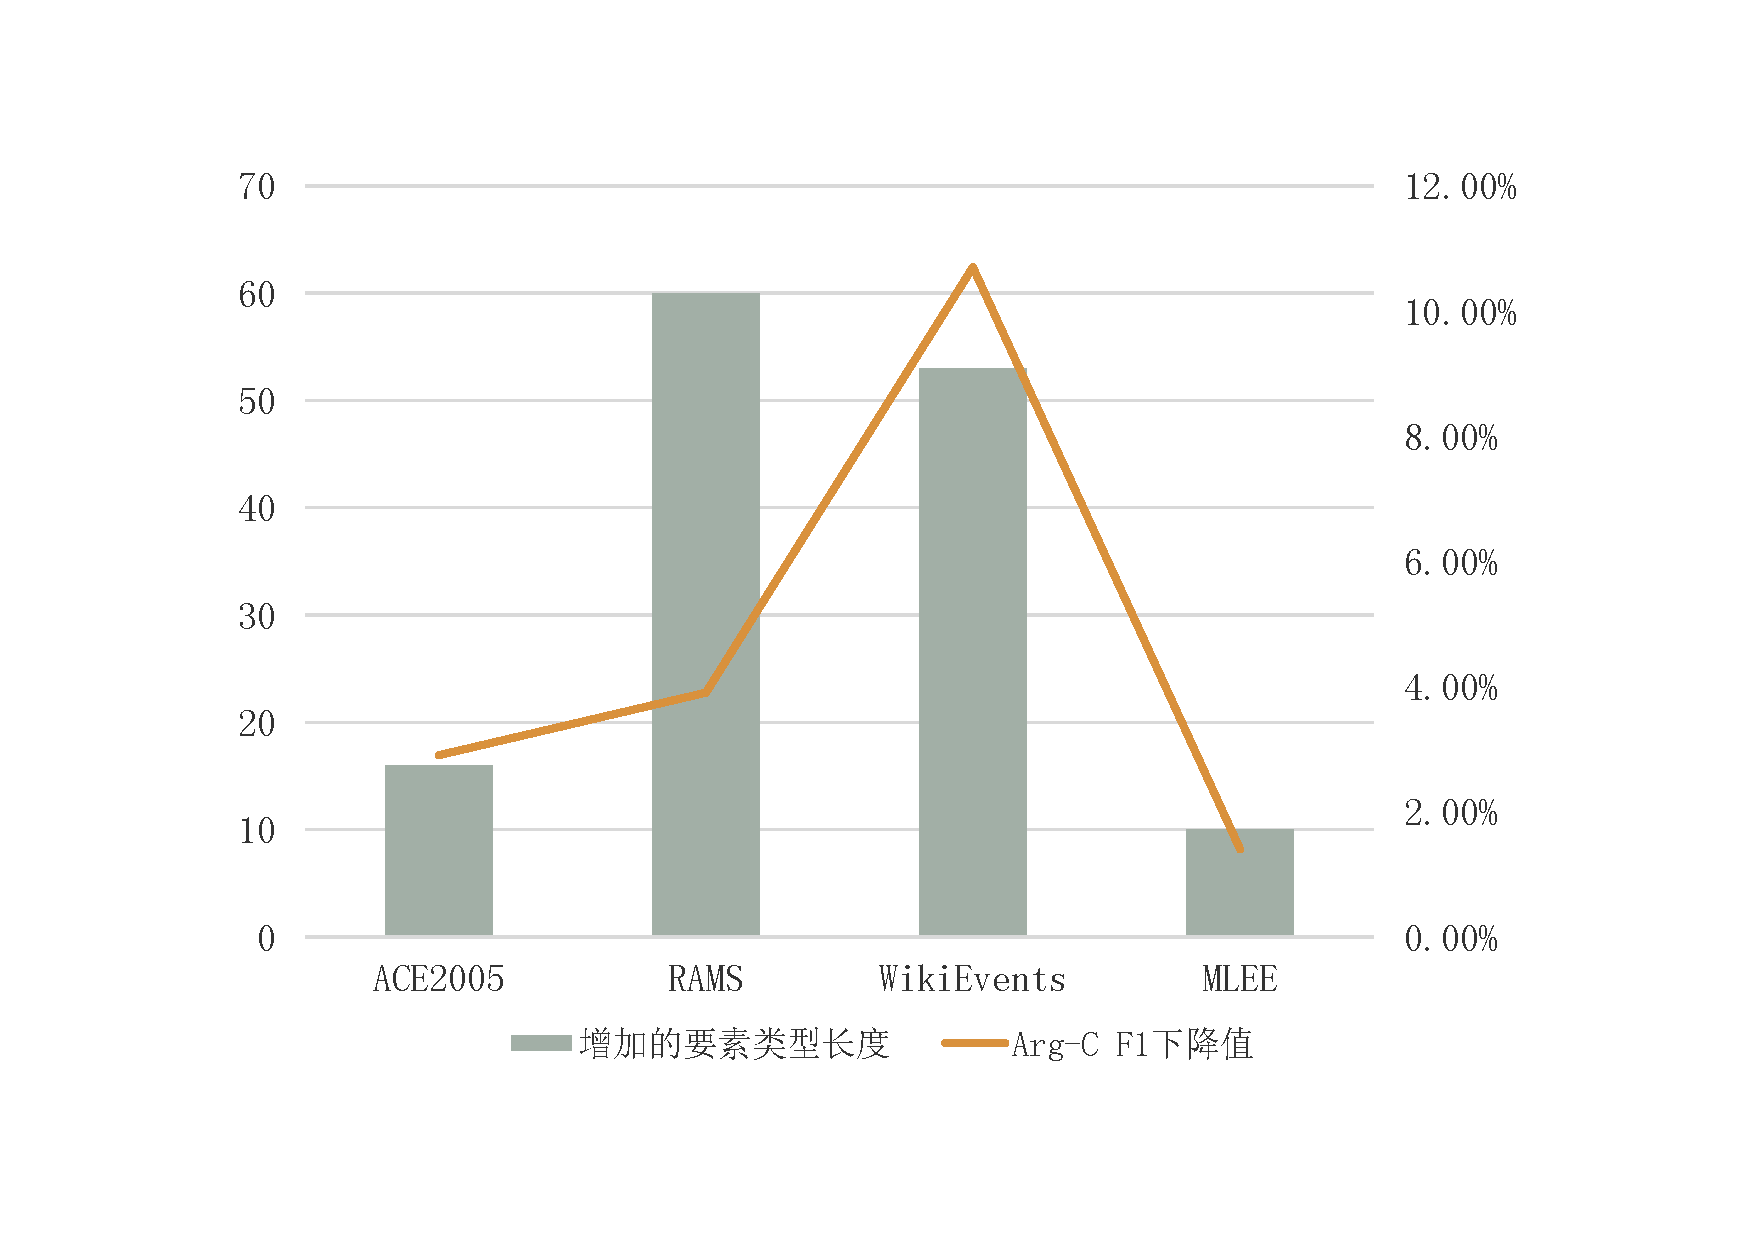
\includegraphics[width=0.55\linewidth]{figures/chap5/relevance.pdf}
\caption{要素类型串接长度与Arg-C F1指标的关联性}
\label{relevance}
\end{figure}

\subsection{单事件/多事件实例性能分析}遵循He等人~\cite{he2023revisiting}的实验设置,本节根据目标抽取事件所在上下文中存在的其他事件的数量(即$|C|$),将每个数据集的测试实例分为两组。当$|C|=0$时,实例中只存在目标抽取事件。如果$|C|>0$,则实例中存在多个事件。然后,基于分组得到各自的统计和性能信息如表\ref{multisingle}所示,其中$[\cdot]$中的值表示对应分组中测试实例的数量,Sep2F-b和Sep2F-l分别表示基于RoBERTa-base和RoBERTa-large的Sep2F模型。值得注意的是,表中其他的基线模型均基于RoBERTa-large进行构建。从表\ref{multisingle}中可以观察到:(1)在两个分组中,基于RoBERTa-large的Sep2F模型在Arg-C F1指标上均超越了之前性能最优的基线。这种性能的提升可以归因于本章所提的分离-融合范式,其同时保留了单事件抽取方式和多事件抽取方式的优点。(2)基于RoBERTa-base的Sep2F模型在WikiEvents和MLEE数据集包含多个事件的实例分组上表现出了令人印象深刻的性能结果,其超越了两个最具性能竞争力的基于RoBERTa-large的SingleE和TabEAE。这验证了本章提出的模型在处理具有多个事件的实例时的良好表现。(3)尽管SingleE和PAIE模型均未利用到跨事件信息,但与PAIE相比,SingleE在所有数据集上均表现出更好的性能结果,其验证了基于多词元链接的模型解决事件要素抽取任务的潜力和优势。

\begin{table*}[htp]
\small
\centering
\caption{四种数据集上单事件/多事件实例对应的Arg-C F1(\%)指标结果}
\begin{tabular}{llcccccccc}
\toprule
\multicolumn{1}{l}{\multirow{3}{*}{模型}} & \multicolumn{2}{c}{ACE2005} & \multicolumn{2}{c}{RAMS} & \multicolumn{2}{c}{WikiEvents} & \multicolumn{2}{c}{MLEE} \\ \cmidrule(lr){2-3} \cmidrule(lr){4-5} \cmidrule(lr){6-7} \cmidrule(lr){8-9}
\multicolumn{1}{l}{} & $|C|=0$ & $|C|>0$ & $|C|=0$ & $|C|>0$ & $|C|=0$ & $|C|>0$  & $|C|=0$  & $|C|>0$ \\ 
\multicolumn{1}{l}{} & [185] & [218] & [587] & [284] & [114] &  [251] &  [175] &  [2025]  \\ \midrule
\multicolumn{1}{l}{SingleE} & 74.8 & 76.0 & 52.9 & 53.3 & 68.4 & 65.5 & 83.1 & 73.8 \\
\multicolumn{1}{l}{MultiE}  & 70.8 & 69.1 & 50.0 & 47.5 & 45.5 & 49.1 & 53.7 & 57.5 \\
\multicolumn{1}{l}{PAIE}  & 71.0 & 73.9 & 52.7 & 52.1 & 65.3 & 65.4 & 78.9 & 70.1 \\
\multicolumn{1}{l}{TabEAE} & 73.4 & 76.1 & 52.9 &  52.5 & 67.3 &  66.2 & 81.1 & 73.6 \\
\midrule
\multicolumn{1}{l}{\textbf{Sep2F-b}} & 72.8 & 74.0 & 52.1 & 52.0 & 66.8 & 69.0 & \textbf{85.5} & 74.9 \\
\multicolumn{1}{l}{\textbf{Sep2F-l}} & \textbf{75.4} & \textbf{78.3} & \textbf{53.2} & \textbf{54.6} & \textbf{68.8} & \textbf{69.5} & 84.3 & \textbf{76.1} \\
\bottomrule
\end{tabular}
\label{multisingle}
\end{table*}

\subsection{消融研究}
本章通过消融研究分析基于RoBERTa-large的Sep2F模型中不同组件的有效性,包括第一阶段融合(First-fold Fusion)、第二阶段融合(Second-fold Fusion)、Blending层(Blending Layer)、文本中存在的其他事件信息(Surrounding Events $C$)和训练损失$\mathcal{L_\textrm{TR}}$(Training Loss $\mathcal{L_\textrm{TR}}$)。根据表\ref{ablation-Sep2F}所示的在Arg-C F1(\%)指标上的消融结果,所有组件均能提升本章提出的Sep2F模型的性能。具体地,可以观察到:(1)如果移除第一阶段融合或第二阶段融合,Sep2F模型在各个数据集上的性能均将下降。这表明两个阶段的融合均对性能提升贡献显著。(2)移除两个阶段中任意一阶段的融合,Sep2F模型在各个数据集上,尤其是WikiEvents和MLEE数据集,取得与之前性能表现最优的事件要素抽取基线模型相当的Arg-C F1指标。这展现了本章提出的模型即使利用简单的融合方法,仍然能在事件要素抽取任务上表现良好,进一步验证了分离-融合范式的优势。(3)当移除Blending层并直接对两个词元链接得分矩阵进行加和,Sep2F模型的Arg-C F1指标在所有数据集上均下降了1.0\%以上,这表明Blending层可以较好地集成不同的词元链接预测分数。(4)如果移除给定目标事件上下文中的其他事件$C$,并在多事件链接构建模块中保留目标事件触发词和在该事件中出现的要素类型之间的链接,则可以发现Sep2F模型在所有数据集上的性能均出现下降,从而明确地证明了跨事件依赖信息对于模型的性能增益。此外,可以发现Sep2F模型在ACE2005和RAMS数据集上性能略有下降,而在WikiEvents和MLEE数据集上则性能下降的更加显著。该观察结果可以归因于表\ref{strategy}中展示的各个数据集中单个实例的平均事件数目的差异。与ACE2005和RAMS数据集相比,本章提出的模型可以利用到WikiEvents和MLEE数据集上更多事件的跨事件信息。因此,与其他两个数据集相比,移除目标事件周围的其他事件信息会导致Sep2F模型在WikiEvents和MLEE数据集上更显著的性能下降。(5)如果移除多事件链接构造模块中的训练损失$\mathcal{L_\textrm{TR}}$(即设置公式\ref{overall_loss}中的训练权重参数$\alpha$为1),则意味着Sep2F模型无法通过调整$\mathcal{L_\textrm{TR}}$而利用到上下文中其他事件的要素类型信息。从消融结果可以看出,由此丢失的跨事件信息使得模型的Arg-C F1指标在ACE2005、RAMS、WikiEvents和MLEE数据集上分别下降了1.2\%、1.8\%、2.3\%和1.9\%。

\begin{table}[htp]
\centering
\caption{四种数据集上关于Arg-C F1(\%)指标的消融研究结果}
\begin{tabular}{lcccc}
\toprule
模型 & ACE2005 & RAMS & WikiEvents & MLEE \\ \midrule
% Sep2F & 73.5 & 52.1 & 68.2 & 75.6 \\ \midrule
% - First-fold Fusion  & 71.5 & 51.3 & 66.1 & 74.0 \\
% - Second-fold Fusion  & 69.6 & 49.7 & 64.3 & 73.9 \\ \midrule
Sep2F & 77.0 & 53.7 & 69.3 & 76.7 \\ \midrule
- First-fold Fusion  & 74.8 & 51.2 & 66.3 & 75.6 \\
- Second-fold Fusion  & 72.5 & 50.2 & 67.8 & 74.2 \\
- Blending Layer  & 75.9 & 52.2 & 66.6 & 75.9 \\
- Surrounding Events $C$  & 76.5 & 52.6 & 66.2 & 74.3 \\
- Training Loss $\mathcal{L_\textrm{TR}}$ & 75.8 & 51.9 & 67.0 & 74.8 \\
\bottomrule
\end{tabular}
\label{ablation-Sep2F}
\end{table}

\subsection{与资源增强模型的性能比较}
本章将Sep2F模型与聚焦于利用跨数据集知识的UnifiedEAE和APE模型作比较,其中APE还额外人工构建了学习重叠知识的提示模版。图\ref{cross-dataset}展示了性能比较结果,其中上半部分的图展示的为基于base版本预训练语言模型的比较,而下半部分的图展示的为基于large版本预训练语言模型的结果。在使用base版本的预训练语言模型时,本章提出的Sep2F模型在所有三个数据集上均优于UnifiedEAE和APE模型。此外,当使用large版本预训练模型时,Sep2F模型在ACE2005和WikiEvents数据集上的性能均优于APE,并在RAMS数据集上也取得与APE相当的Arg-C F1指标。因此,可以得知尽管参与比较的基线受益于额外的训练资源和人为设计的经验知识,本章提出的模型在使用不同版本预训练语言模型时仍能在绝大部分数据集上实现最佳性能,进一步证明了其在事件要素抽取任务上的优越性。

\begin{figure}[htp]
\centering
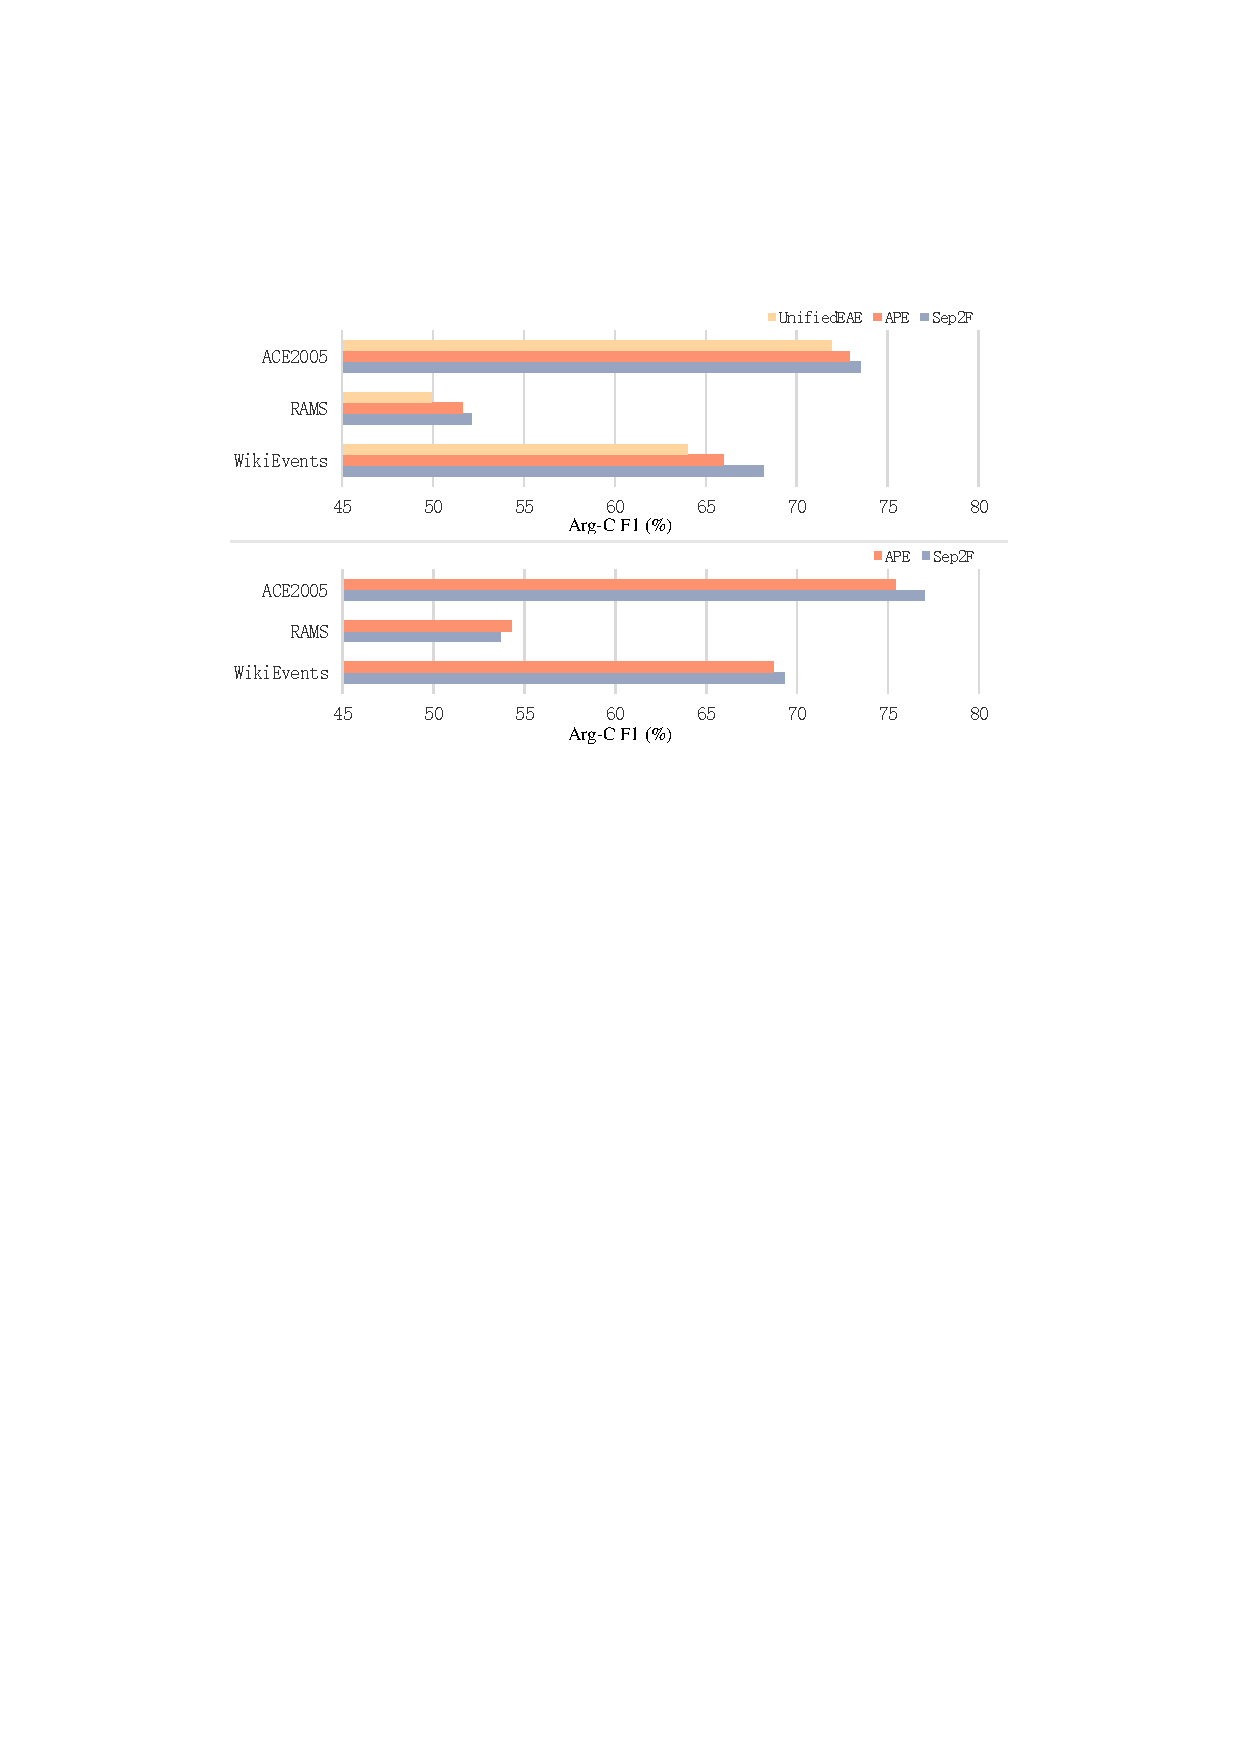
\includegraphics[width=1\linewidth]{figures/chap5/comparison.pdf}
\caption{三种数据集上Sep2F与资源增强模型的性能结果对比} 
% The upper figure illustrates the comparison using base-version PLMs, while the bottom figure shows the results with large-version PLMs.}
\label{cross-dataset}
\end{figure}

\subsection{案例研究}
本章节基于WikiEvents数据集中的一个具体实例进行定性的案例分析。图\ref{case-sep2f}展示了本章提出的Sep2F模型和SingleE模型在该实例上的事件要素抽取结果,其不同事件的触发词被不同颜色标记,且这两个模型均基于RoBERTa-large进行构建和训练。可以观察到,SingleE模型未能预测出由“booming”触发的$Attack$事件中的两个事件要素,但Sep2F模型给出了正确的预测结果。本章推测其原因为Sep2F模型可以利用到由“killed”触发的事件中的要素类型信息。同样,由于跨事件要素类型$Destroyer$提供了重要的依赖信息提示,Sep2F模型避免了事件触发词“death”的干扰,将“He”的要素类型识别为$Killer$而不是$Victim$,但SingleE模型给出了错误的抽取结果。

\begin{figure}[htp]
\centering
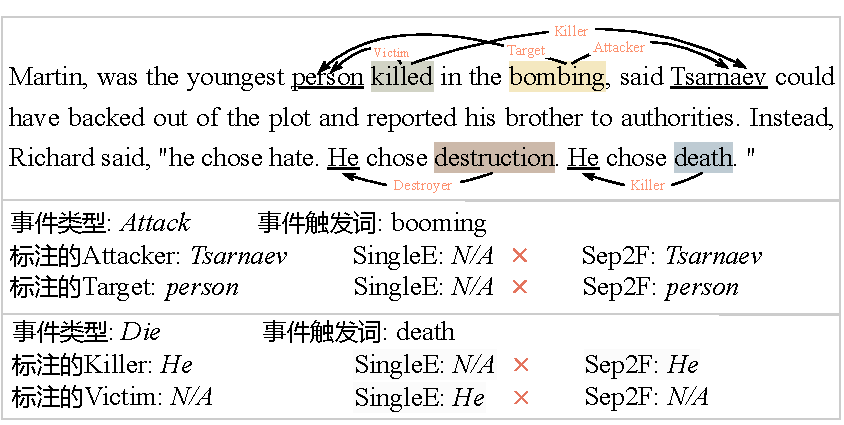
\includegraphics[width=0.8\linewidth]{figures/chap5/case-sep2f.pdf}
\caption{WikiEvents数据集上的案例分析}
\label{case-sep2f}
\end{figure}

\subsection{训练权重超参数分析}
本章研究公式\ref{overall_loss}中训练权重$\alpha$对于Sep2F模型性能的影响。表\ref{alpha_Sep2F}展示了不同$\alpha$取值下Sep2F模型在各个数据集上的Arg-C F1性能指标,可以观察到本章提出的Sep2F模型在不同数据集上均性能稳定,证明了其良好的鲁棒性。

\begin{table}[htp]
\centering
\caption{四种数据集上不同$\alpha$取值对应的Arg-C F1(\%)指标结果}
\begin{tabular}{ccccc}
\toprule
训练权重$\alpha$ & ACE2005 & RAMS & WikiEvents & MLEE \\ \midrule
0.5  & 76.1 & \textbf{53.7} & 68.6 & 76.6 \\
0.6  & 76.8 & 53.0 & 68.7 & 76.4 \\
0.7  & 76.7 & 53.1 & \textbf{69.3} & 76.6 \\
0.8  & \textbf{77.0} & 52.7 & \textbf{69.3} & \textbf{76.7} \\
0.9  & 76.4 & 52.8 & 67.9 & 76.4 \\
% 1.0  & 75.8 & 51.9 & 67.0 & 74.8 \\
\bottomrule
\end{tabular}
\label{alpha_Sep2F}
\end{table}

\section{本章小结}

本章提出了一种新颖的多词元链接事件要素抽取模型。具体地,提出了两个链接模块来分离跨事件信息的获取和目标事件的要素抽取过程。此外,提出了一种新的两阶段融合模块,以确保获取的跨事件信息能够有效地增益目标事件的要素抽取。因此,本章所提模型利用了跨事件依赖线索并保留了单事件抽取方式的优点。本章在四个不同级别的基准数据集上进行了充分实验,结果表明提出的模型在所有数据集上均取得了事件要素抽取的最优性能。